\section{Dynamic Bipedal Locomotion in the Real World}\label{sec:experiments}


We now extensively evaluate the obtained versatile policies for walking, running, and jumping in the real world. 
All of these policies are able to effectively control the robot in the real world without further tuning after being trained in simulation. 
Moreover, the main objective of the experiments is to evaluate two fundamental aspects of the proposed method: (1) the obtained policies' \textit{adaptivitiy} to the actual robot dynamics in the real world by effectively controlling the real robot to achieve the assigned tasks, as in simulation; and (2) the policies' \textit{robustness} in addressing different uncertainties in the real world by leveraging various learned and tasks.




\subsection{Walking Experiments}
We now examine the versatile walking policy on Cassie. 
The following experiments are conducted by a \textit{single} controller. As we will see, the obtained walking policy shows consistent control performance on the robot hardware over a long timespan with notable robustness and compliance.


\subsubsection{Tracking Performance}\label{subsec:tracking_performance_walking}
The policy demonstrates the capacity to reliably track varying, fast-changing commands, with consistent control performance over a long period that is more than a year. Such a result showcases the adaptivity of the proposed policy that adapts to the dynamics of the real robot, as discussed below.  


\paragraph{Variable Commands}


\begin{figure*}[!htp]
    \centering
    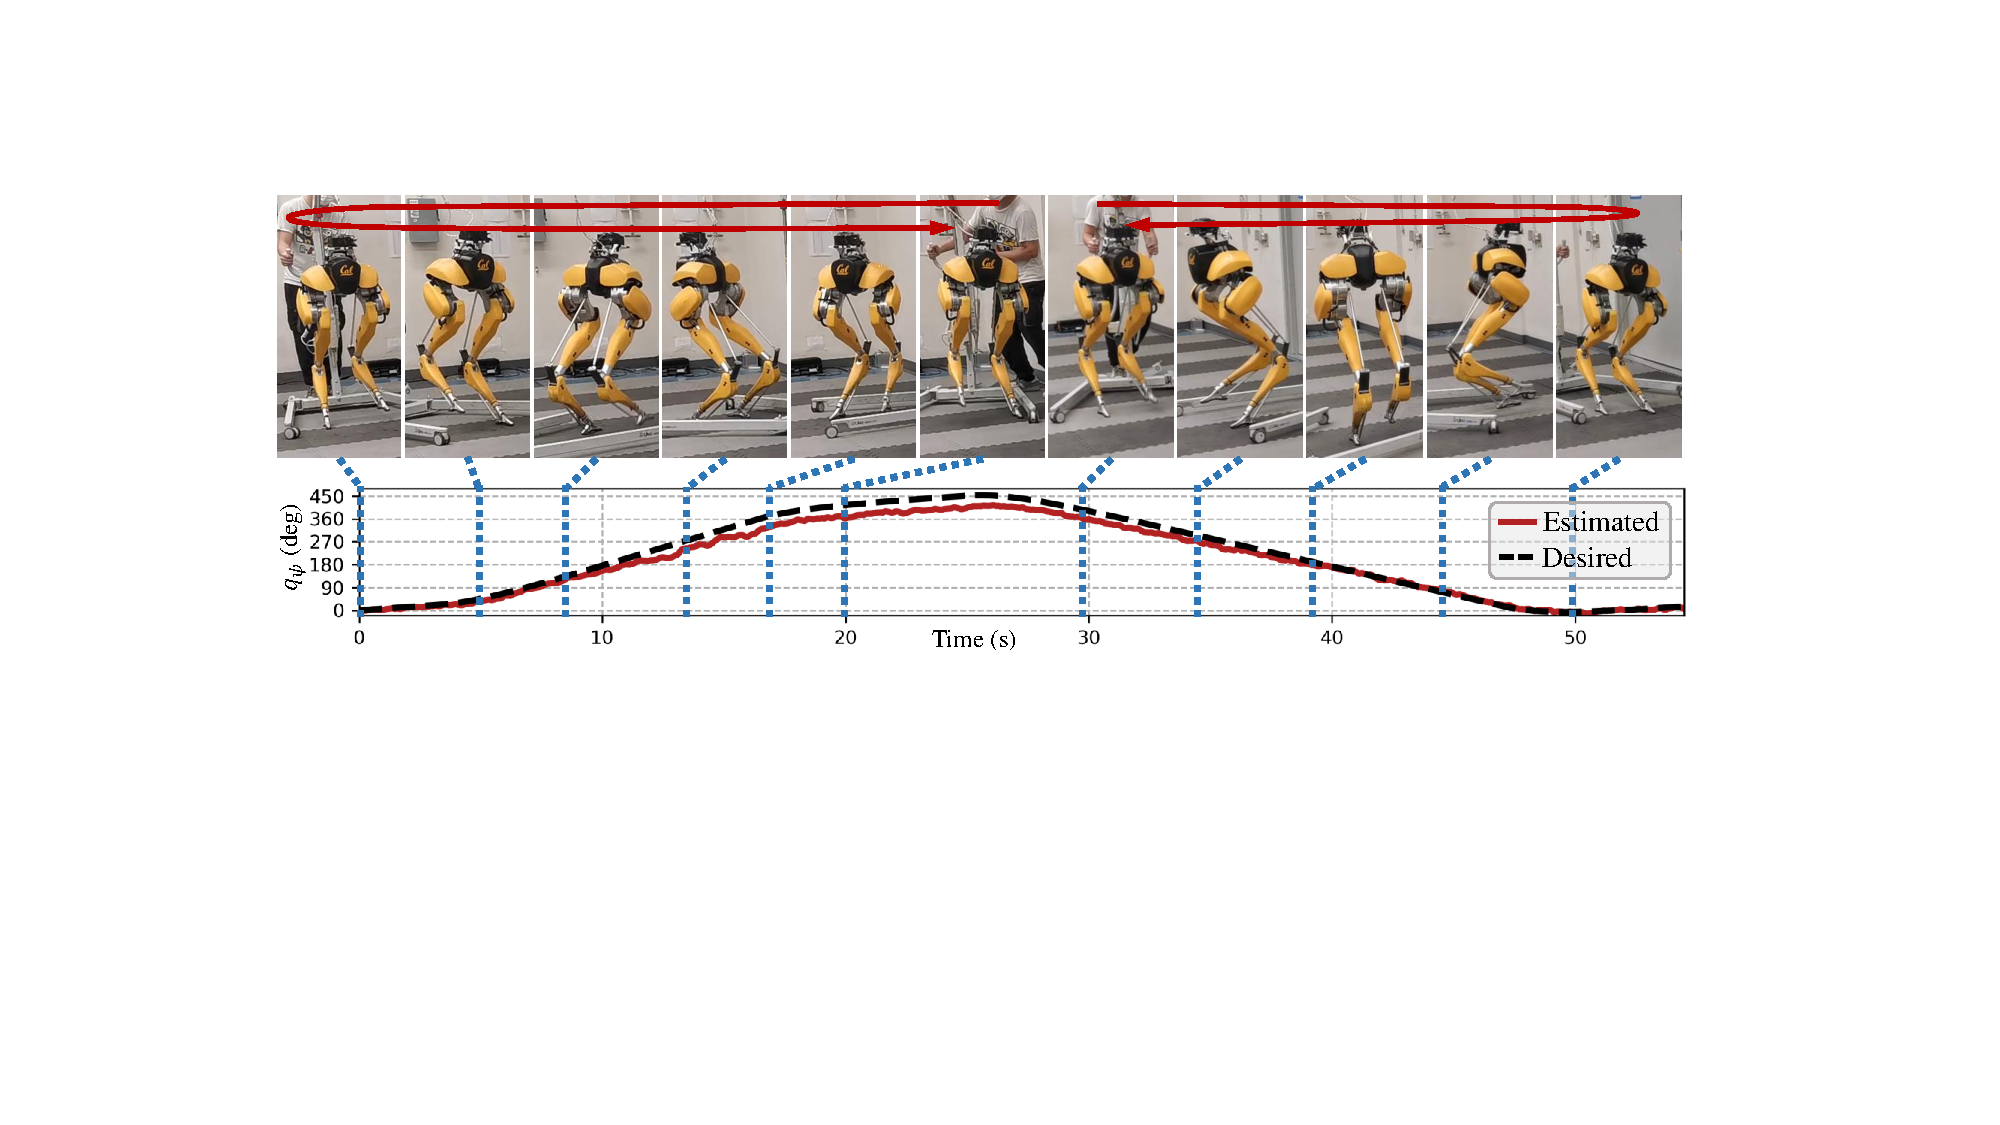
\includegraphics[width=\linewidth]{figures/turning.pdf}
    \caption{A snapshot from the real world demonstrating the robot reliably tracking various turning yaw commands $q^d_{\psi}$ using the same controller used in Fig.~\ref{fig:variable_cmd}. Both the desired and actual turning angles are recorded in the lower part, with dashed lines matching the corresponding frames in the real world. The robot can execute full turns in both counterclockwise and clockwise directions.}
    \label{fig:turning}
\end{figure*}


\begin{figure*}[!htp]
\centering
\begin{subfigure}{0.345\linewidth}
  \centering
  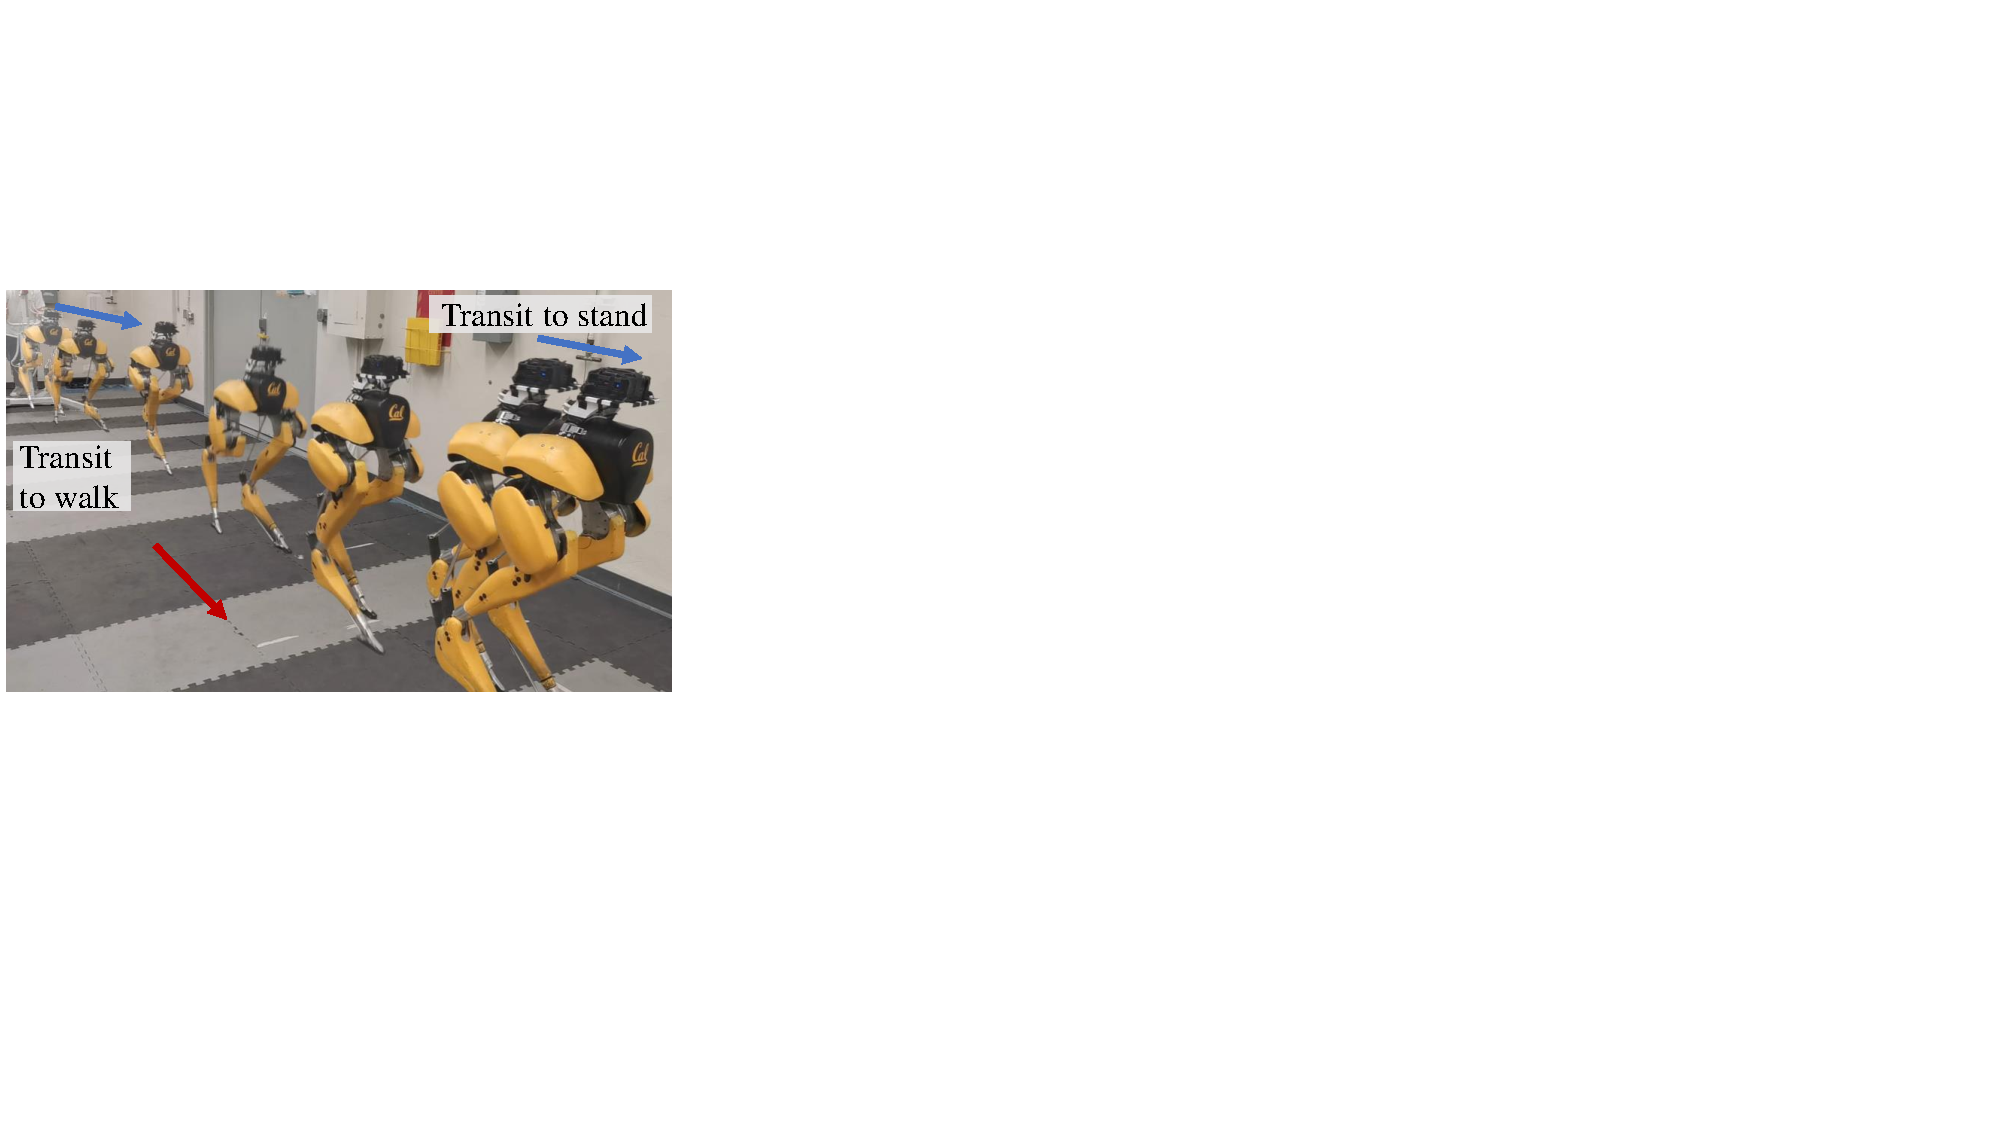
\includegraphics[width=\linewidth]{figures/fast_walking_forward_snapshot.pdf}
  \caption{Fast Forward Walking}
  \label{subfig:fast_forward}
\end{subfigure}
\begin{subfigure}{0.345\linewidth}
  \centering
  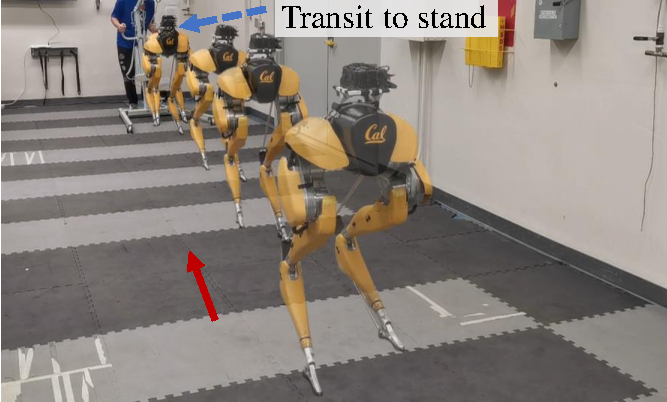
\includegraphics[width=\linewidth]{figures/fast_walking_backward_snapshot.pdf}
  \caption{Fast Backward Walking}
  \label{subfig:fast_backward}
\end{subfigure}
\begin{subfigure}{0.2725\linewidth}
  \centering
  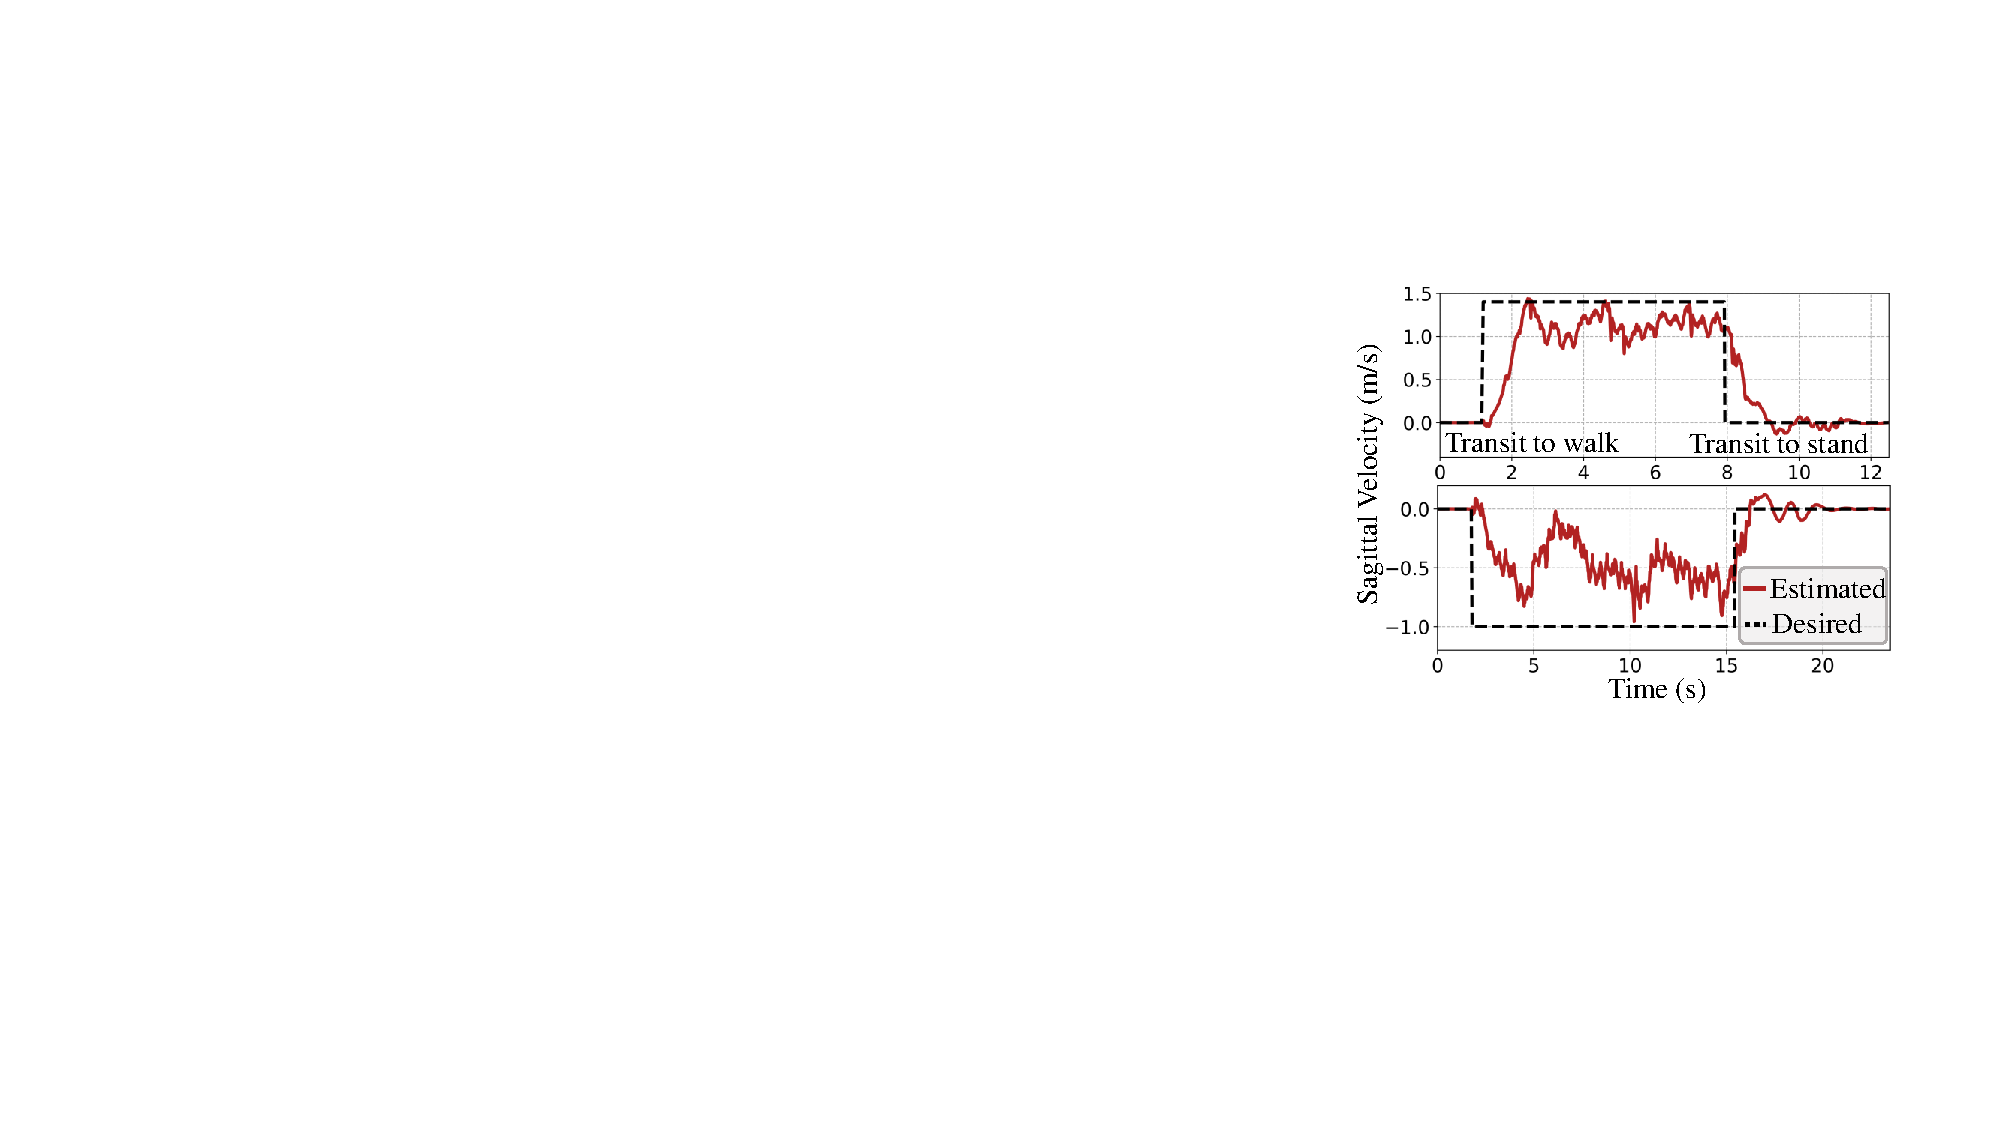
\includegraphics[width=\linewidth]{figures/fast_walking_log.pdf}
  \caption{Corresponding Recorded Data}
  \label{subfig:fast_walking_log}
\end{subfigure}
\caption{Snapshots of the robot transiting from standing to fast forward walking (Fig.~\ref{subfig:fast_forward}) or backward walking (Fig.~\ref{subfig:fast_backward}) and back to standing, using the same walking policy. Earlier frames appear more faded. The robot's commanded and actual sagittal velocities are recorded in Fig.~\ref{subfig:fast_walking_log}. This demonstrates the robot's capability to quickly switch from a stationary stance to dynamic fast walking and smoothly transition back to standing with a single command, even during dynamic maneuvers like fast walking.}
\label{fig:fast_walking}
\end{figure*}


As recorded in Fig.~\ref{subfig:variable_cmd}, the walking policy demonstrates efficient control over the robot's following of diverse commands, including variations in sagittal and lateral velocities ($\dot{q}_{x,y}$) and walking height ($q_z$). 
Throughout the test, the tracking errors, evaluated by Mean Absolute Error (MAE), remain reasonably low. 
The MAE in the $(\dot{q}_x, \dot{q}_y, q_z)$ are (0.10 m/s, 0.10 m/s, 0.06 m) respectively.
Additionally, as indicated in Fig.~\ref{fig:turning}, the policy exhibits reliable control, enabling the robot to accurately track varying turning commands, either clockwise or anti-clockwise.



\paragraph{Consistency over a Long Timespan}
The robot hardware, especially for bipedal robots, keeps changing due to wear and tear over time. 
For instance, joint friction might vary due to the impacts during operation, and these changes can accumulate due to the bipedal robot's large number of DoFs and over extended periods. 
Consequently, controllers dependent on the control gains tuned on hardware, like most model-based controllers, often require manual updates to deal with these hardware changes.
In contrast, our proposed RL-based walking policy can adapt to changing robot dynamics and control the robot without the need for tuning on the hardware. 
This adaptivity is evident as the policy consistently performs well over extended periods, maintaining its ability to track variable commands even after 325 and 492 days, as showcased in Fig.~\ref{subfig:variable_cmd_0630} and Fig.~\ref{subfig:variable_cmd_1214}, respectively. 
Compared with the test conducted earlier (Fig.~\ref{subfig:variable_cmd}), the changes of the tracking errors (MAE) in $(\dot{q}_x, \dot{q}_y, q_z)$ during these two tests are ($+0$ m/s, $-0.02$ m/s, $+0$ m) and ($+0.01$ m/s, $-0.01$ m/s, $-0.01$ m), respectively, over a relatively long testing timespan (over 2 minutes) with different combinations of commands.
Despite significant accumulated changes in the robot's dynamics over this period, the same controller from Fig.~\ref{subfig:variable_cmd} continues to effectively manage varying walking tasks with only minimal tracking error degradation.






\paragraph{Fast Walking}
In addition to previously demonstrated moderate walking speeds, the policy exhibits the ability to control the robot to perform fast walking maneuvers, both forwards and backwards, as shown in Fig.~\ref{fig:fast_walking}. 
The robot can transition from a standstill to rapidly achieve a forward walking speed with an average velocity of $1.14$ m/s to track the command of $1.4$ m/s, quickly returning to a standing position as commanded, as shown in Fig.~\ref{subfig:fast_forward} with data recorded in Fig.~\ref{subfig:fast_walking_log}.
Notably, during the transition from a stance pose with zero speed, the robot can quickly swing its legs forward with a considerable amount of acceleration while maintaining gait stability to follow the step-input command. 
Similar capacity is observed in the context of fast backward walking (Fig.~\ref{subfig:fast_backward}), where the robot seamlessly shifts from a standing pose to perform a backward walking gait with an average velocity of $-0.5$ m/s, achieving the specified $-1$ m/s walking task before promptly returning to a standing position upon command.



\begin{figure*}[t]
\centering
\begin{subfigure}{0.495\linewidth}
  \centering
  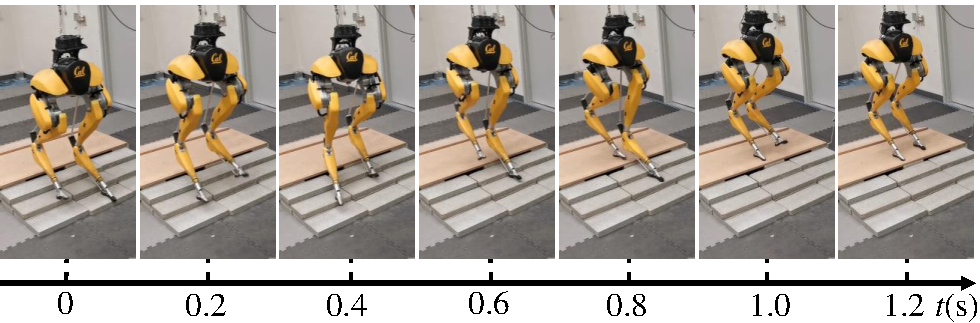
\includegraphics[width=\linewidth]{figures/walking_stairs.pdf}
  \caption{Walking Backwards on Stairs}
  \label{subfig:walking_stairs}
\end{subfigure}
\begin{subfigure}{0.495\linewidth}
  \centering
  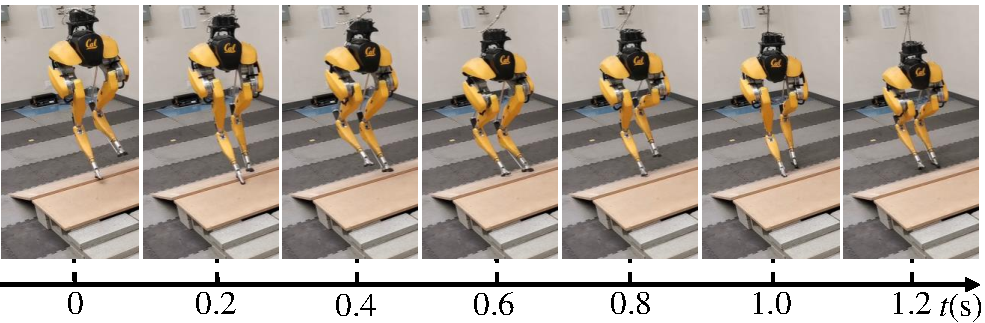
\includegraphics[width=\linewidth]{figures/walking_slope.pdf}
  \caption{Walking Backwards on Slope}
  \label{subfig:walking_slope}
\end{subfigure} 
\caption{Snapshots of the robot Cassie performing a robustness test by walking \emph{backwards} over small varied terrains such as stairs (Fig.~\ref{subfig:walking_stairs}) or slope (Fig~\ref{subfig:walking_slope}). Snapshots are aligned with time stamps. Although the policy wasn't specifically trained for terrain deviations, it successfully maintains stable walking gaits and robustness in the face of ground elevation changes in real-world scenarios as recorded in these set of snapshots.}
\label{fig:walking_terrain}
\end{figure*}

\begin{figure*}[t]
\centering
\begin{subfigure}{0.65\linewidth}
  \centering
  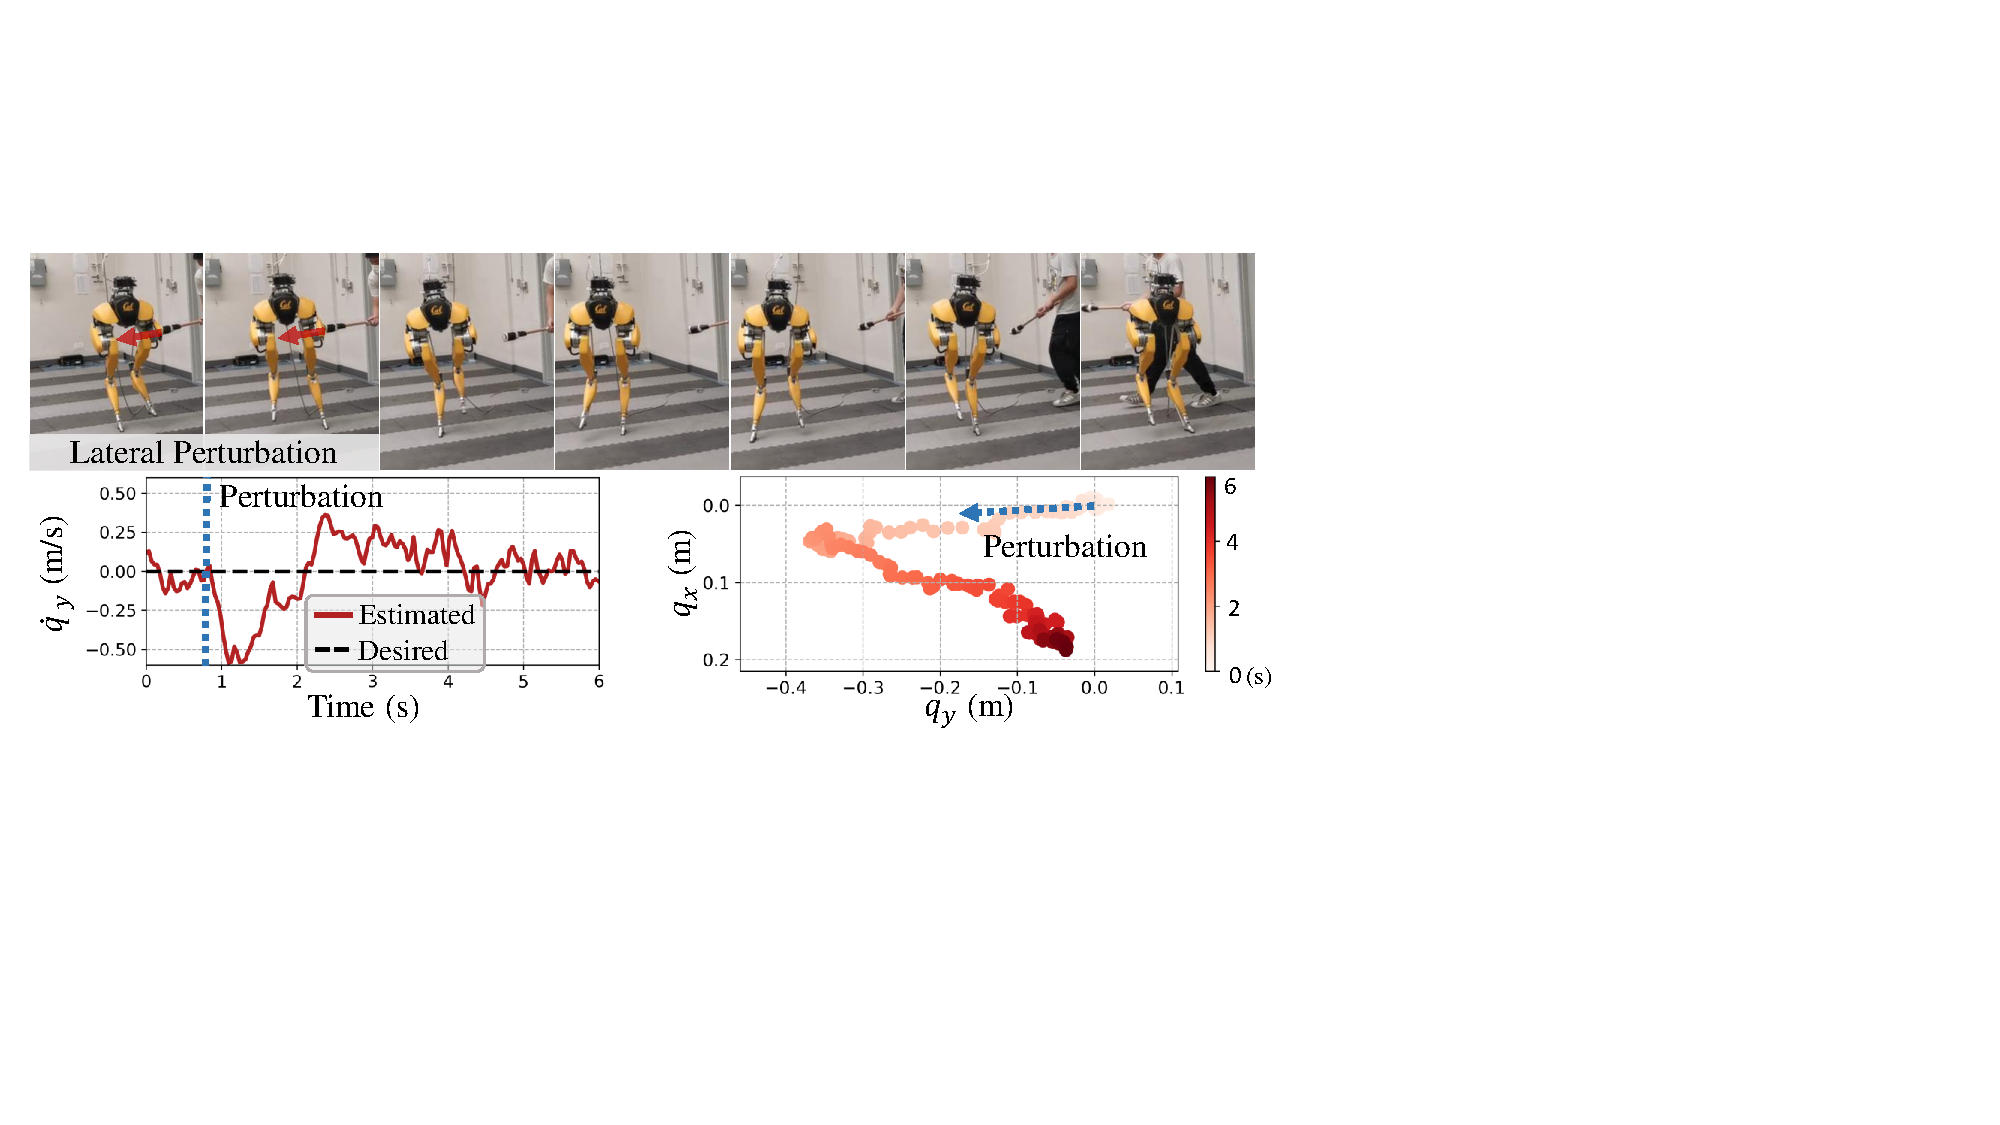
\includegraphics[width=\linewidth]{figures/push_recovery_rl.pdf}
  \caption{Recovery maneuvers using the proposed RL-based controller from lateral perturbation}
  \label{subfig:push_recovery_rl}
\end{subfigure}
\begin{subfigure}{0.31\linewidth}
  \centering
  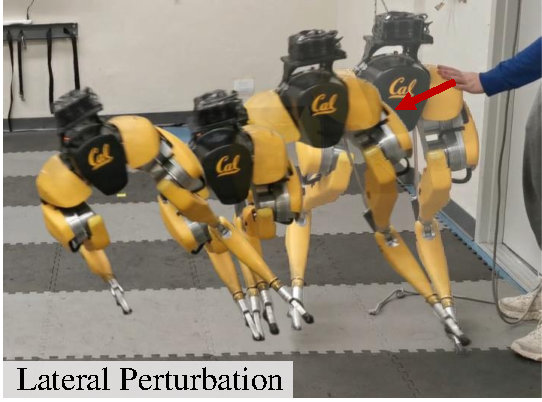
\includegraphics[width=\linewidth]{figures/push_recovery_mpc.pdf}
  \caption{A model-based controller that failed to recover the robot from lateral perturbation}
  \label{subfig:push_recovery_mpc}
\end{subfigure}  
\caption{Robustness test of the robot walking against unknown perturbations. Using the proposed RL-based versatile policy, as seen in Fig.\ref{subfig:push_recovery_rl}, the robot, despite being pushed laterally and accelerated to $-0.5$ m/s, still maintains a stable walking gait and compensates such a lateral impulse by walking in the opposite direction. The corresponding lateral velocity $\dot{q}_y$ is recorded in the lower part of the figure. Additionally, the planar position $(q_y,q_x)$ is estimated, with points appearing in progressively darker colors as they are recorded later in time. In contrast, using a model-based controller provided by Cassie's manufacturer (Fig.~\ref{subfig:push_recovery_mpc}), the robot crashes after a similar lateral push.}
\label{fig:walking_perturb}
\end{figure*}


\begin{figure*}[t]
\centering
\begin{subfigure}{0.8\linewidth}
  \centering
  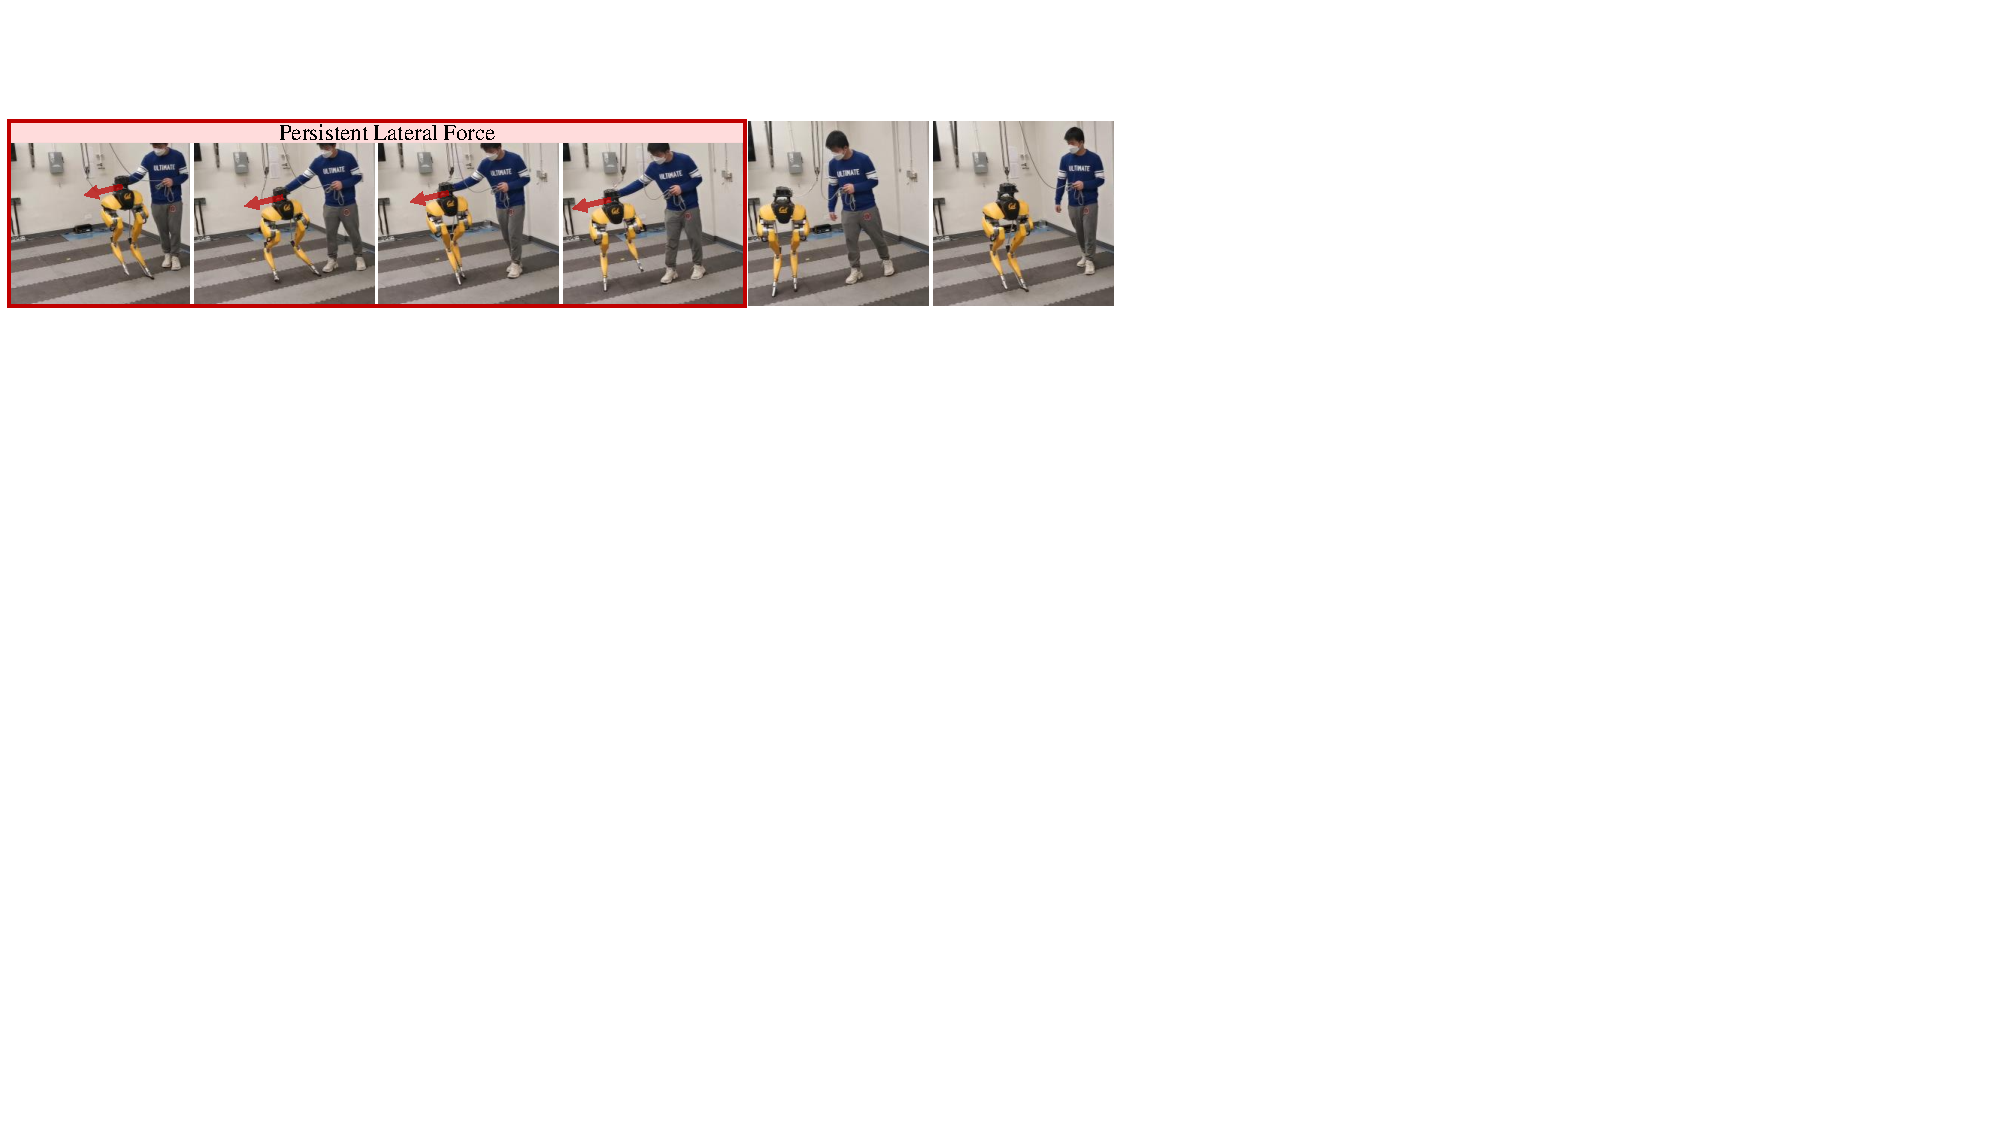
\includegraphics[width=\linewidth]{figures/compliance_normalheight.pdf}
  \caption{Staying compliant to a persistent lateral force at a normal walking height}\label{subfig:compliance_normalheight}
\end{subfigure}
\begin{subfigure}{0.8\linewidth}%0.495
  \centering
  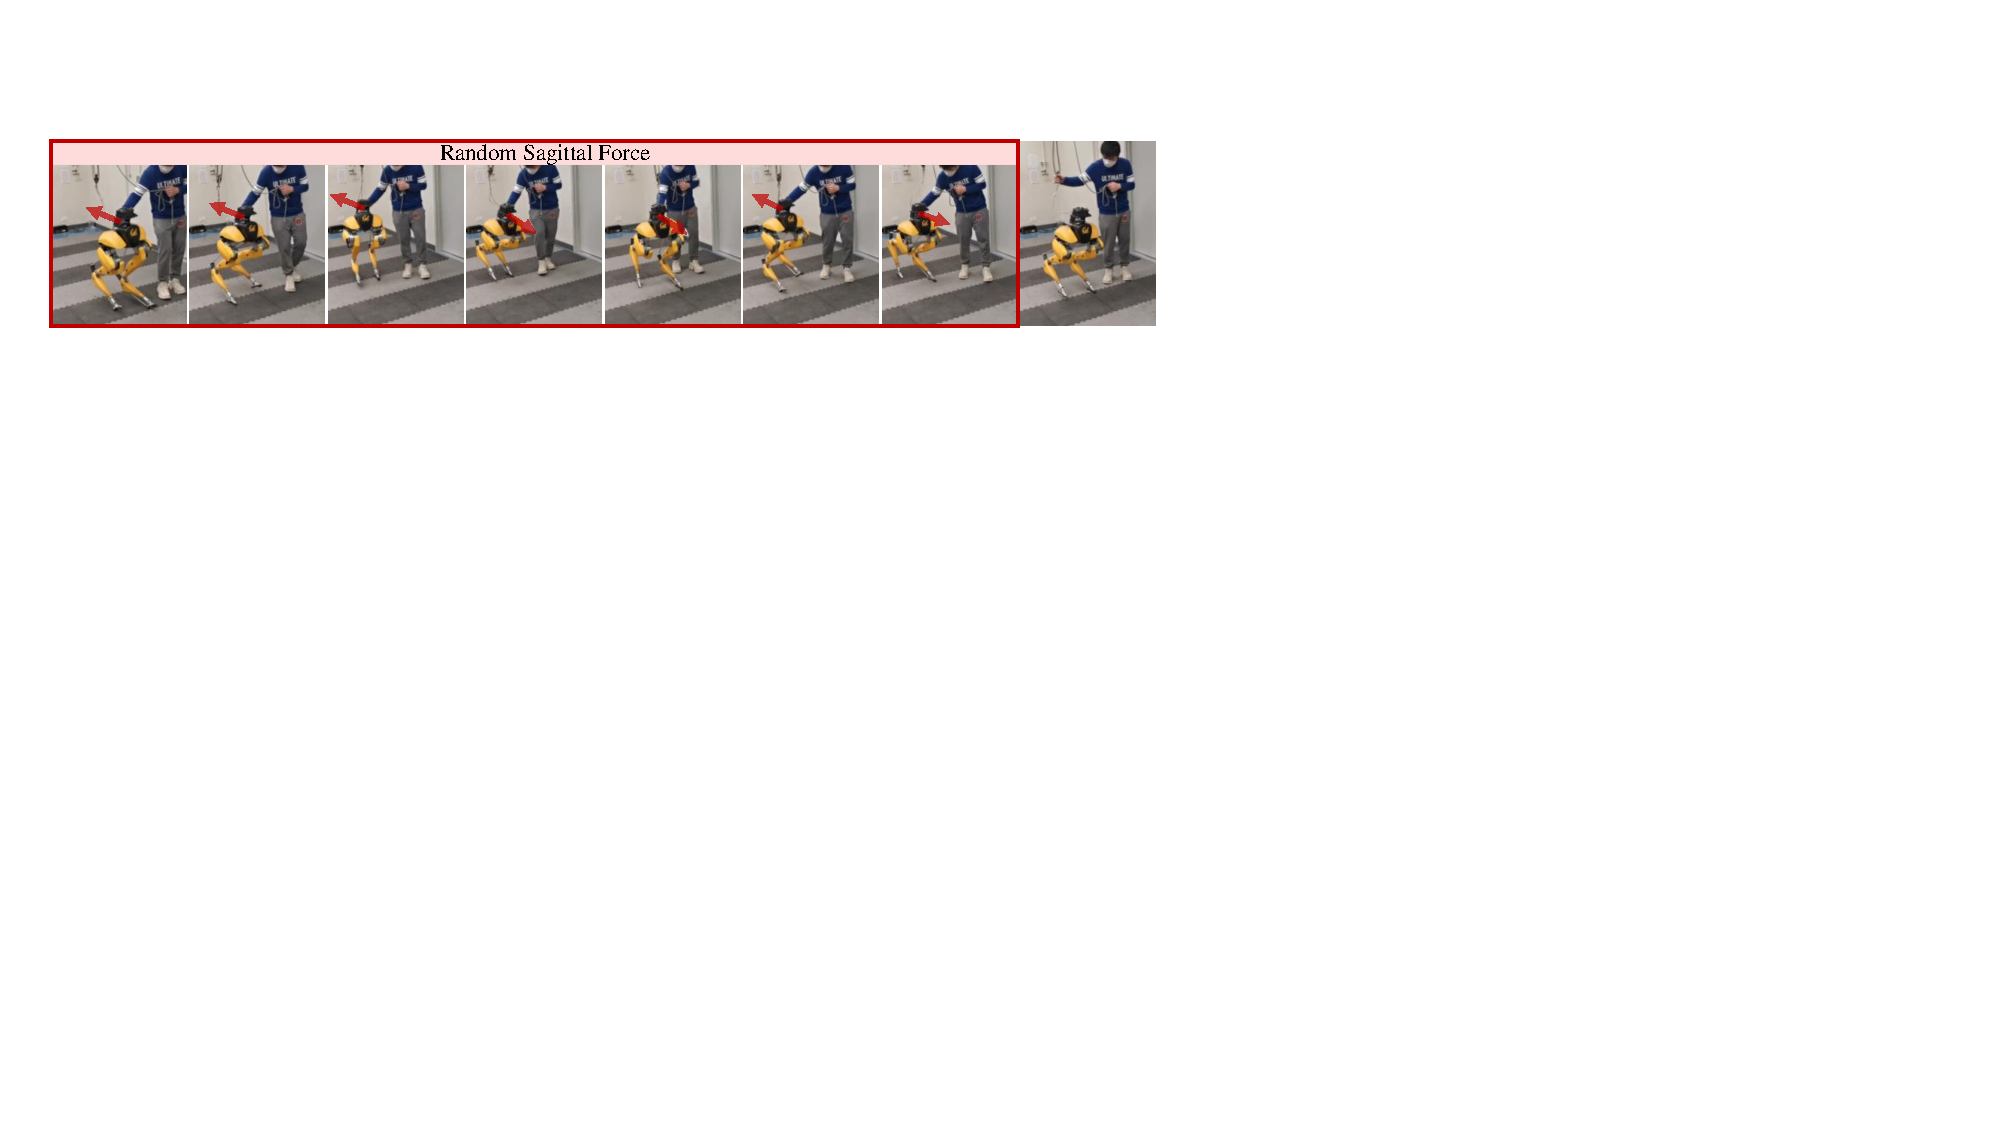
\includegraphics[width=\linewidth]{figures/compliance_lowerheight.pdf}
  \caption{Staying compliant to a persistent and random sagittal force at a low walking height}\label{subfig:compliance_lowerheight}
\end{subfigure} 
\caption{Snapshots of the compliance test using the proposed versitale walking policy in the real world. The red arrows illustrate the direction of the applied force. In Fig.~\ref{subfig:compliance_normalheight} where the robot is walking at a normal height, a human applies a persistent (longer than 3 seconds) lateral force on Cassie's base and drags the robot to its right. In Fig.~\ref{subfig:compliance_lowerheight} where the robot is at a low walking height, a human exerts a persistent but random force on the robot's base and drags the robot back and forth in the sagittal direction. In these tests, the robot demonstrates compliance by walking along the persistent external force direction without losing balance, although being commanded to walk in place. After the force is removed, the robot returns to the commanded task.}
\label{fig:walking_compliance}
\end{figure*}






\subsubsection{Robust Walking Maneuvers}
We further test the robustness of the walking policy, and the proposed policy shows notable robustness in addressing various changes in the environment, as showcased below.

\paragraph{Uneven Terrains (Untrained)} 

Although the walking policy has not been specifically trained for traversing uneven terrain in simulation, it displays considerable robustness to varying elevation changes during deployment.
As depicted in Fig.~\ref{fig:walking_terrain}, the robot can effectively walk \emph{backward} on small stairs or declined slopes. 
It's noteworthy that the robot lacks any terrain elevation sensors. 
Such ability stems from the policy's robustness to the change of contact timing or wrench while walking on varying elevations, facilitated by \emph{not} requiring explicit estimation or control of the contact in the controller.



\paragraph{Robustness to Random Perturbations}
In this test, we evaluate the robustness of the proposed versatile walking policy under two types of external perturbations: (1) impulse perturbation whose elapsed time is less than 1 second; (2) persistent perturbation that lasts more than 3 seconds (longer than the length of controller's I/O history). 

For the impulse perturbation case, we introduced external perturbations over a short timespan from various directions to the robot while walking. 
As an example recorded in Fig.~\ref{subfig:push_recovery_rl}, a substantial lateral perturbation force is applied to the robot while walking in place, causing a significant lateral velocity peak of 0.5 m/s. 
Despite this force, the robot swiftly recovers from the lateral deviation. 
As recorded in Fig.~\ref{subfig:push_recovery_rl}, the robot adeptly moves in the opposite lateral direction, effectively compensating for the perturbation and restoring its stable in-place walking gait.





During the test for persistent perturbation, a human exerts a persistent force on the robot base and drags the robot in random directions while the robot is commanded to walk in place.  
Examples can be seen in Fig.~\ref{subfig:compliance_normalheight}, a persistent lateral dragging force is applied to Cassie's base while the robot is walking at normal height. 
In another test where the robot is walking at a lower height as shown in Fig.~\ref{subfig:compliance_lowerheight}, the robot's base is subject to a persistent force with its direction changing randomly in the sagittal direction. 
During these tests, without losing balance, the robot shows compliance to these external forces by following the directions of these forces, despite being commanded to walk in place. 
These compliance experiments demonstrate the advantages of the proposed RL-based policy in controlling the bipedal robot for potential applications like safe human-robot interaction.

More scenarios, including more impulse perturbations and persisting random perturbations, are recorded in the accompanying Vid. 3 in Table~\ref{tab:video_list}.
In all conducted tests, the robot demonstrates its robustness, being consistent with the results observed in the simulation validation in Sec.~\ref{sec:multi_skill}.
The underlying reason behind this lies in the robot's extensive learning of various tasks such as lateral, forward, backward walking, turning, and more.
This task randomization enables the robot to generalize the knowledge gained while learning from various tasks to recover from deviations occurring in the current commanded task.



\begin{figure*}[t]
\centering
\begin{subfigure}{\linewidth}
  \centering
  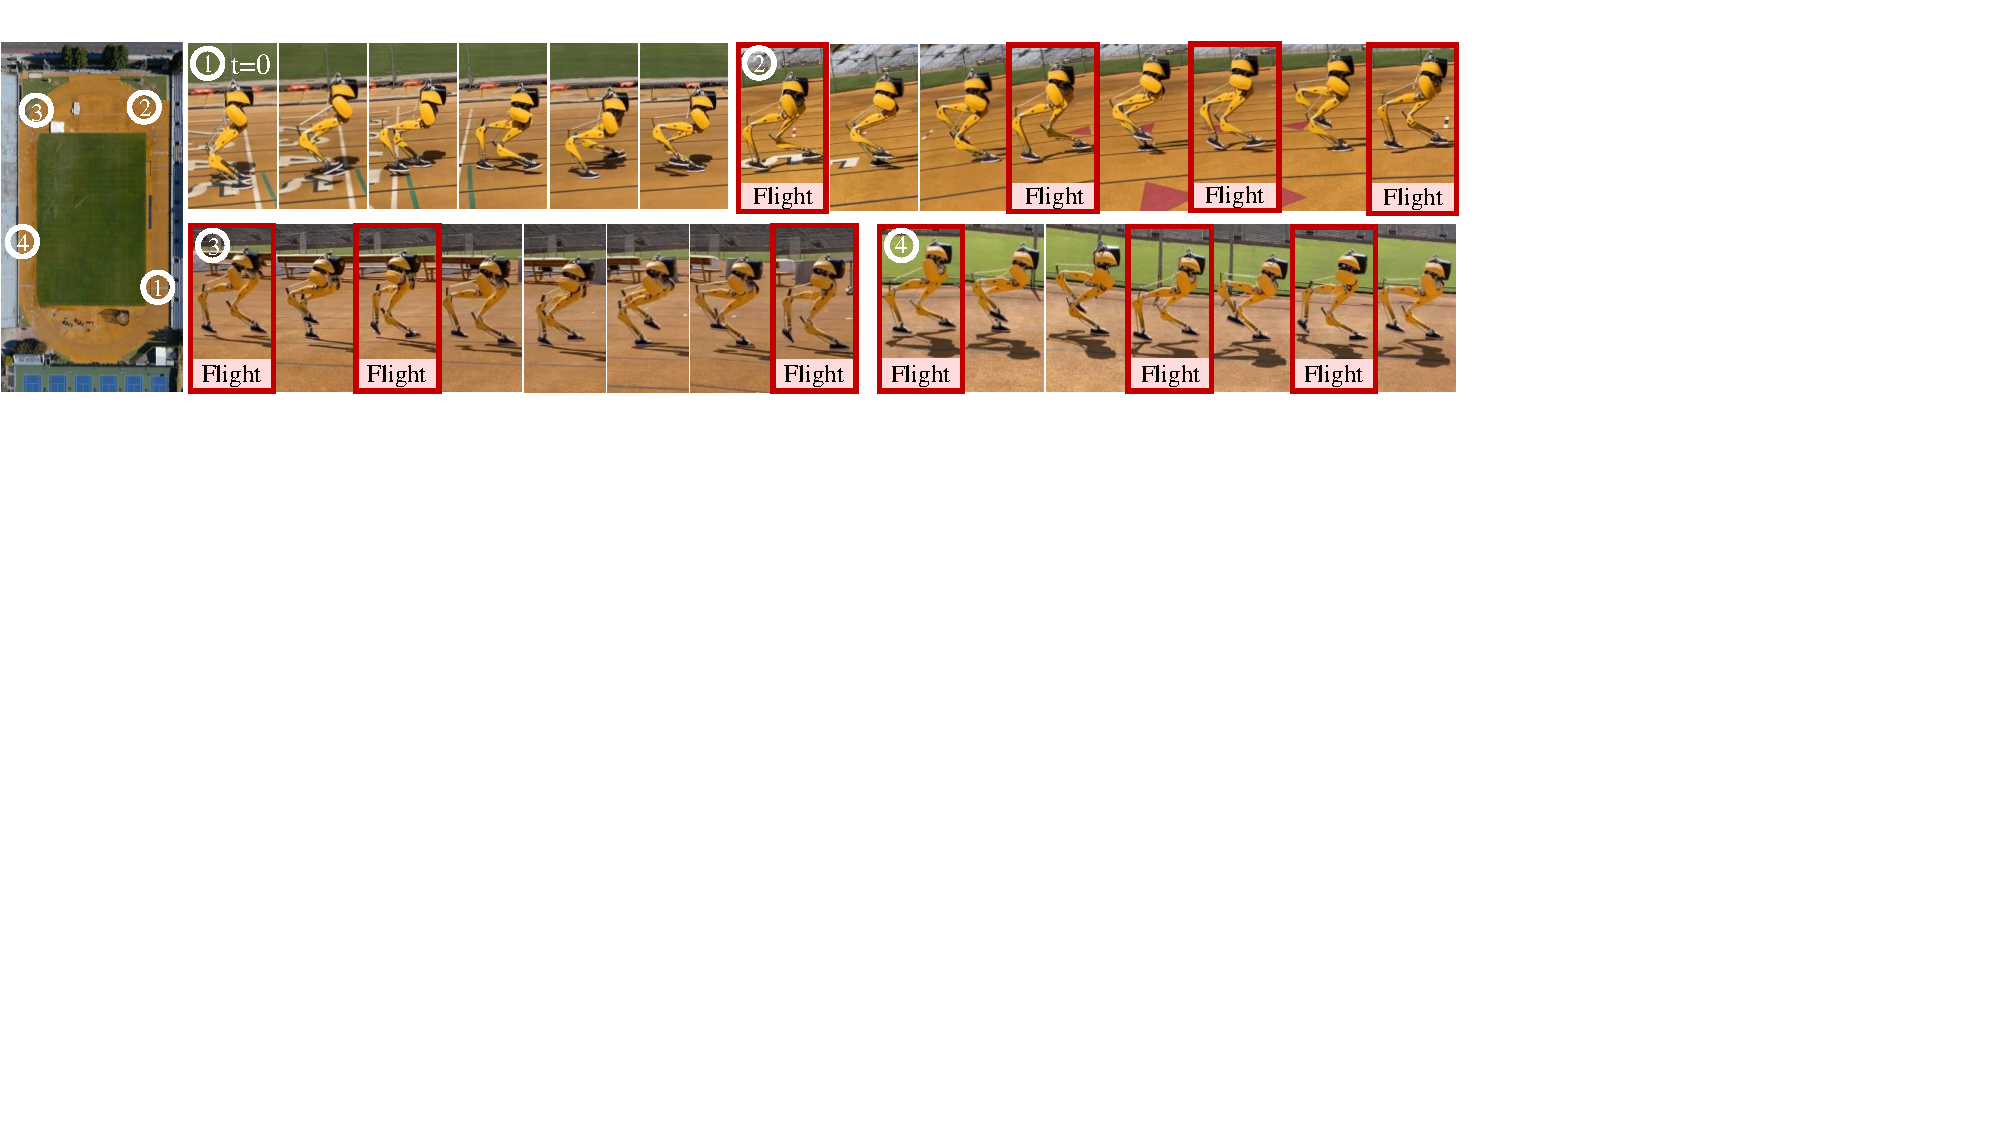
\includegraphics[width=\linewidth]{figures/run_400_snapshot.pdf}
  \caption{Snapshot of 400-meter dash. The number matches the snapshot of the robot and the corresponding position on the running track.}
  \label{subfig:run_400_snapshot}
\end{subfigure}
\begin{subfigure}{\linewidth}
  \centering
  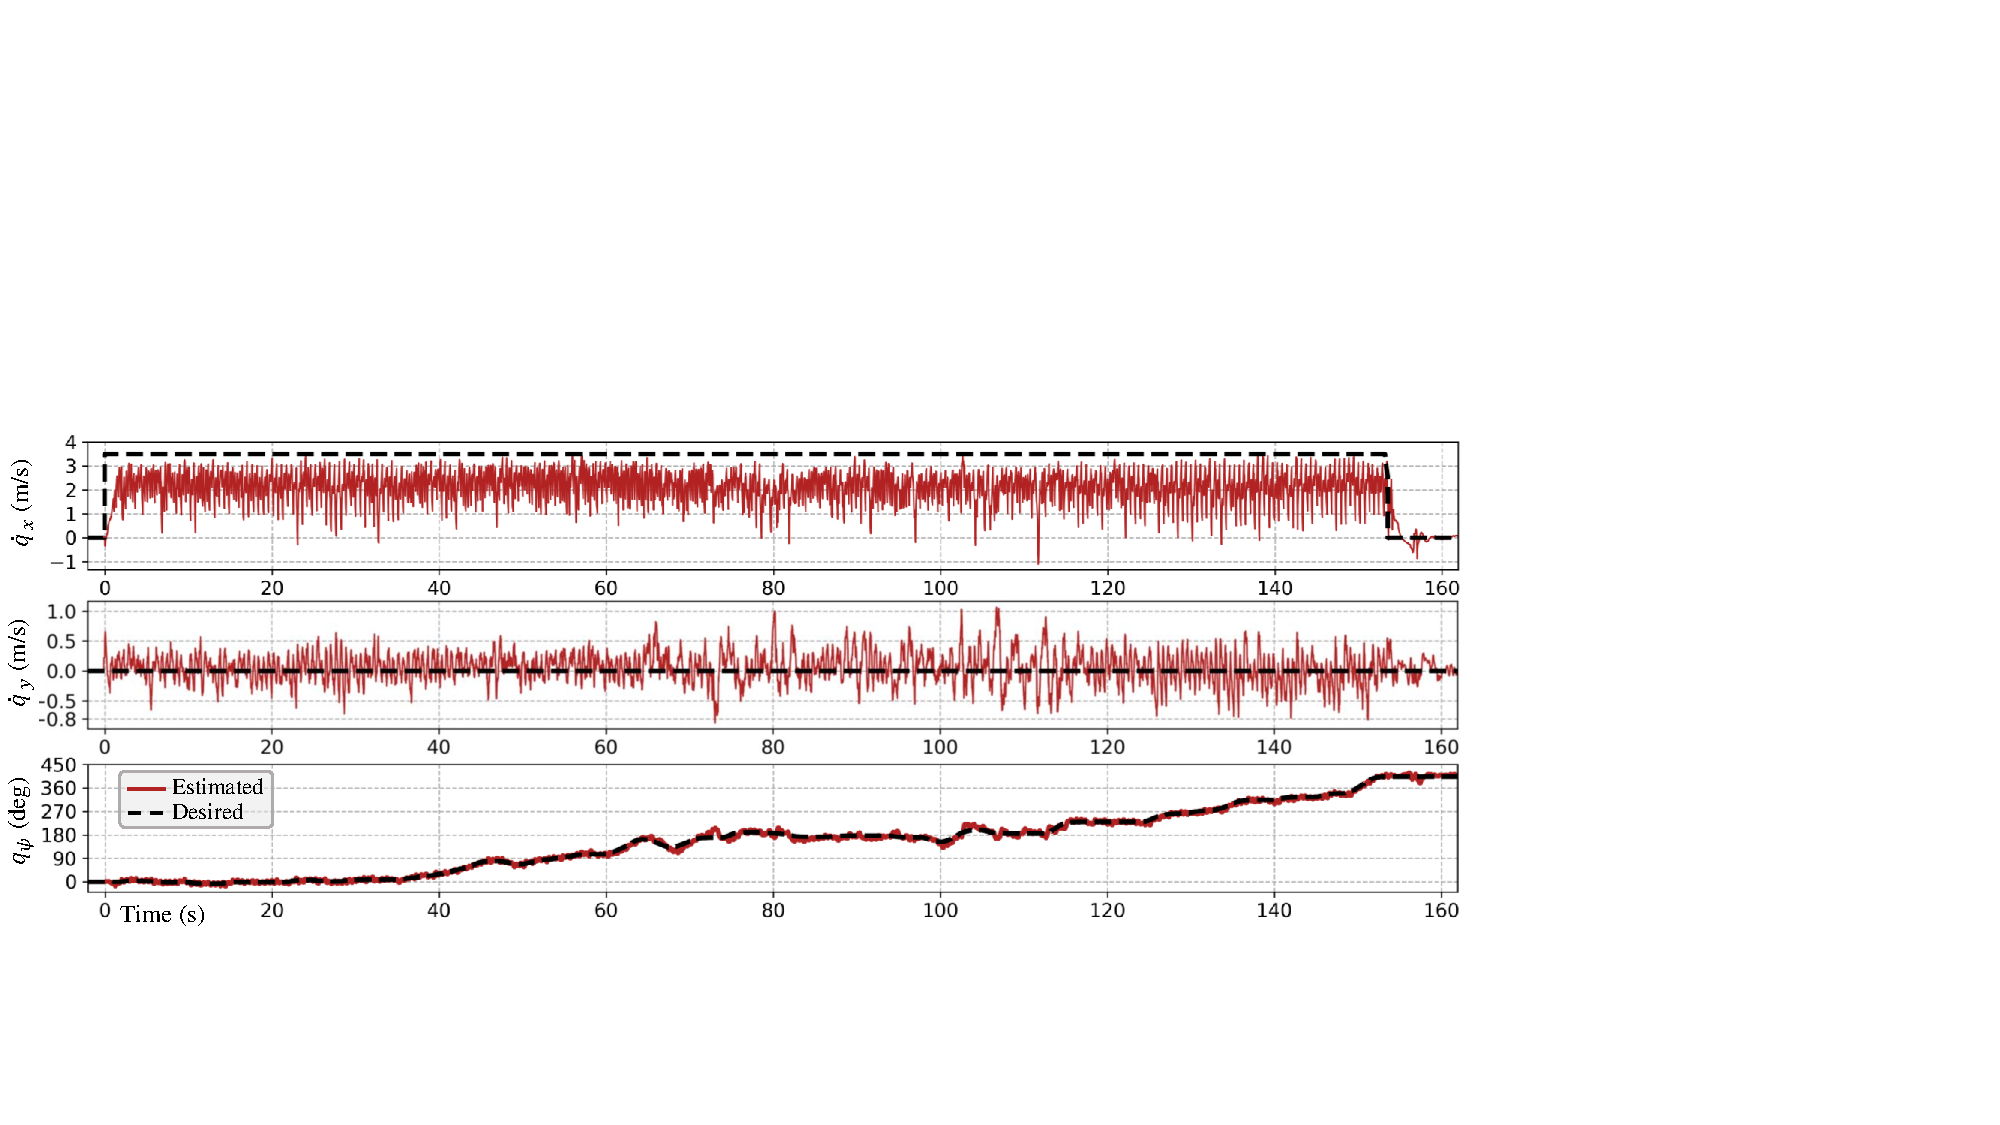
\includegraphics[width=\linewidth]{figures/run_400_log.pdf}
  \caption{Recorded data during the 400-meter dash. The robot's sagittal velocity $\dot{q}_x$, lateral velocity $\dot{q}_y$ and turning yaw angle $q_\psi$ are shown.}
  \label{subfig:run_400_log}
\end{subfigure}  
\caption{Utilizing a versatile running policy we developed, Cassie successfully completed a 400-meter dash in the bipedal robot regime with a time of 2 minutes and 34 seconds. The dash is completed in the Edwards Stadium at UC Berkeley. This is made possible using a single running policy that enabled the robot to transition from a standing pose to fast running gaits of 2.15 m/s at average and 3.54 m/s at peak. The robot also maintains that speed with an average lateral speed of 0.05 m/s (with zero lateral speed command) throughout the dash. Additionally, the robot is able to accurately follow varying turning commands with an average tracking error (MAE) of 5.95 degrees. This precise turning command tracking was crucial for the successful completion of the 400-meter dash, as it required the robot to reliably turn while running.
During running, we consistently observed noticeable flight phases as examples seen in Fig.~\ref{subfig:run_400_snapshot}. The robot is also able to transit back to standing after it finished the dash, as recorded in the sagittal velocity log (Fig.~\ref{subfig:run_400_log}) and Vid. 2 in Table~\ref{tab:video_list}.}    
\label{fig:400run}
\end{figure*}









\paragraph{Comparison with a Model-based Controller}
We underline the advantages of the proposed walking policy by comparing it with a model-based walking controller, specifically, a model-based controller utilized by the company that manufactured Cassie.
As shown in Fig.~\ref{subfig:push_recovery_mpc}, when the robot is controlled by this model-based controller and subjected to lateral perturbation, this controller fails to maintain control, resulting in a crash. This is because that the model used in the controller does not consider the external perturbation (which is also hard to estimate), and the model-based controller can not deal with such a large modeling error.  
The model-based controller also fails to stabilize the robot during a persistent perturbation test. 
These experiments are recorded in Vid. 3 in Table~\ref{tab:video_list}.
A systematic perturbation test for legged robots was carried out in a very recent work by \cite{van2024revisiting} and it would be interesting to incorporate such tests more widely. 
However, this is beyond the scope of this paper. 
Furthermore, as shown in the video, the model-based controller causes obvious lateral drifts on the robot (before the human operator perturbed it) when it is commanded to track a zero speed without manual gain tuning, while the proposed RL policy shows better tracking performance (that keeps the robot walking in-place) without training using real-world data. However, the model-based controller results in less and favorable stomping force than the RL policy. 
We hope these experiments could help the readers better understand the pros and cons of model-based optimal control and model-free RL methods for bipedal locomotion control.





\subsubsection{Summary of Results}
In summary, the versatile walking policy derived from the proposed method is able to effectively control the bipedal robot Cassie to perform diverse tasks in the real world and be consistent over a long time of usage (more than a year). 
The results show that the robot can track different walking velocities, varying walking heights, turn in different directions, and perform fast walking and transition to and from standing.
The policy also exhibits substantial robustness in the face of challenges such as changes in terrain elevation and external perturbations (including impulse and random but persistent forces).


\begin{figure*}[!htp]
\centering
\begin{subfigure}{0.305\linewidth}
  \centering
  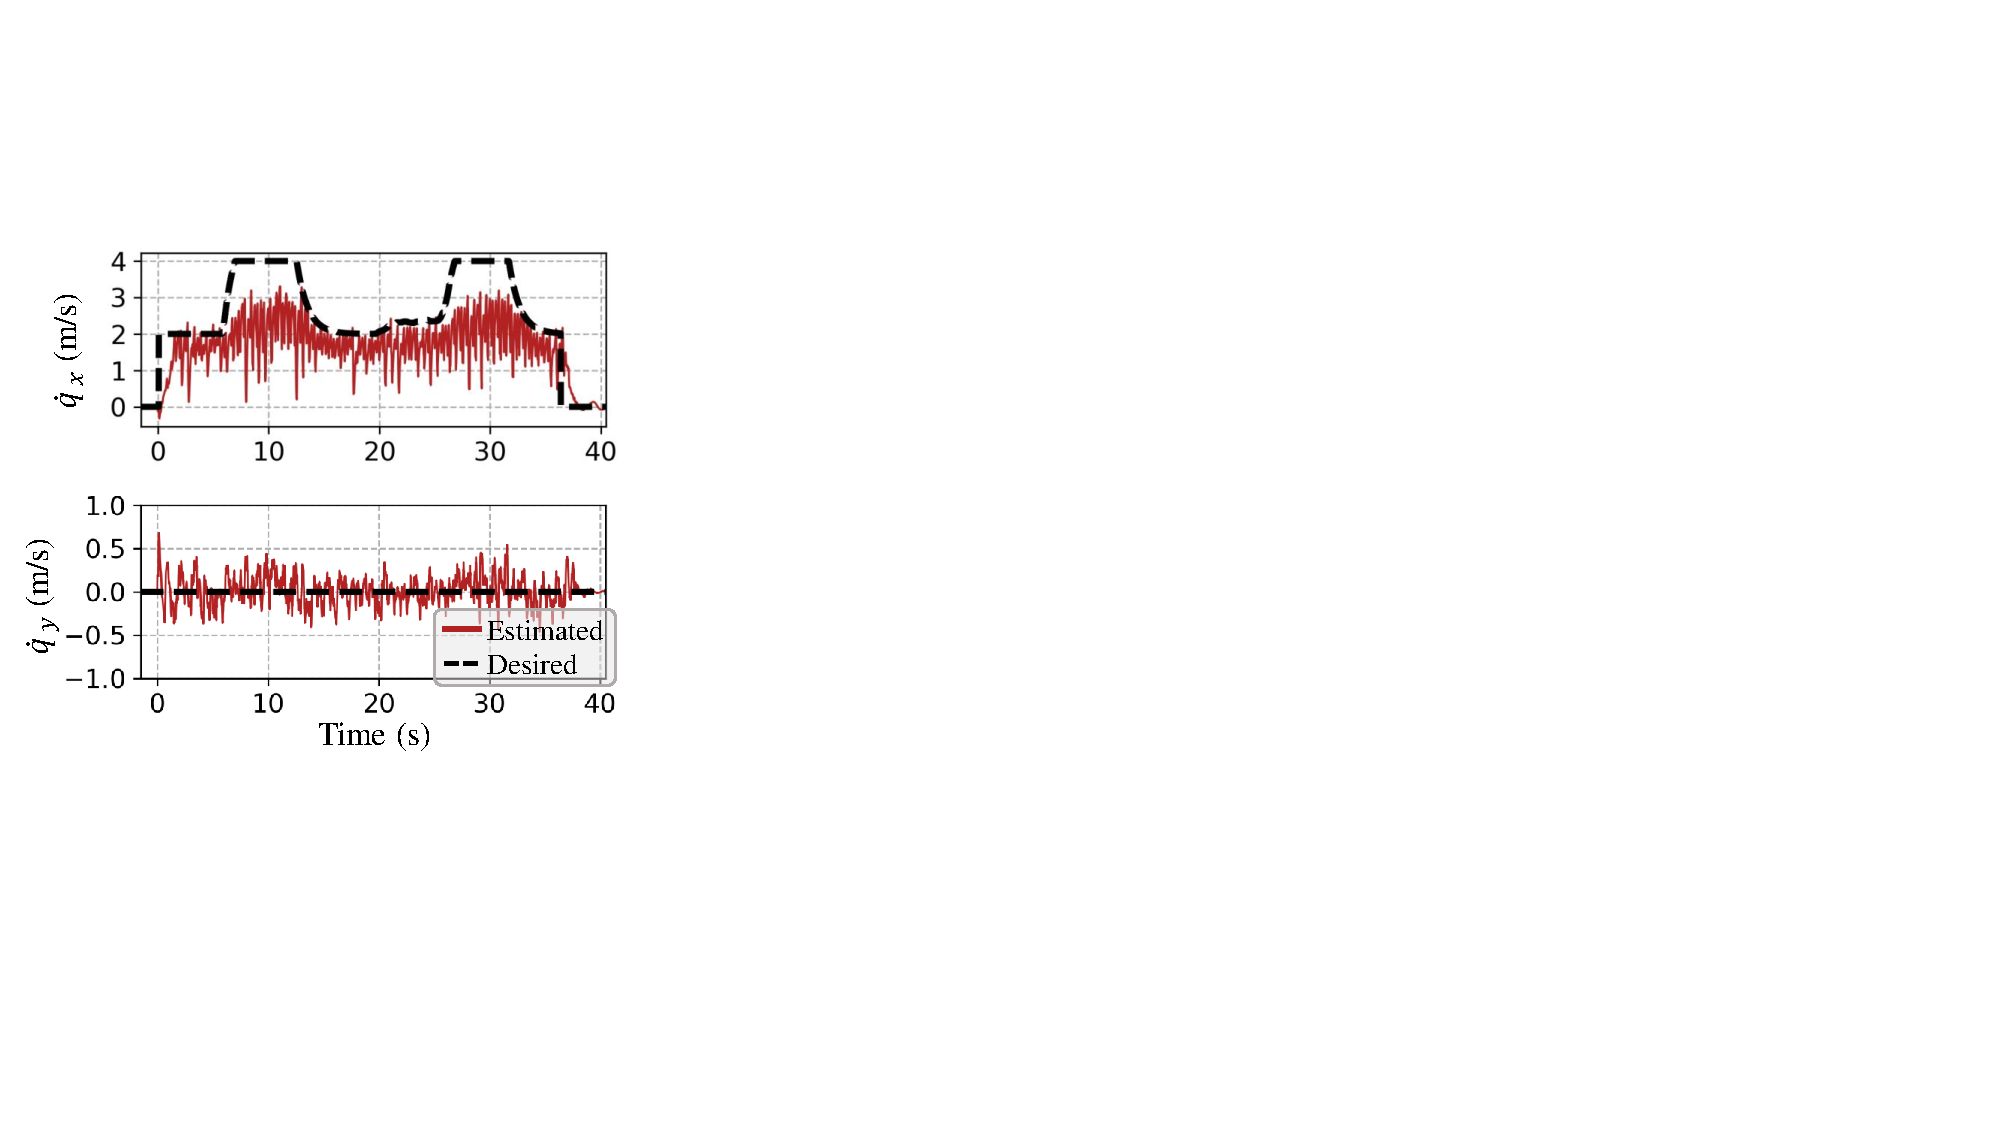
\includegraphics[width=\linewidth]{figures/run_variablevx.pdf}
  \caption{Tracking variable sagittal velocity during running}
  \label{subfig:run_variablevx}
\end{subfigure}
\begin{subfigure}{0.305\linewidth}
  \centering
  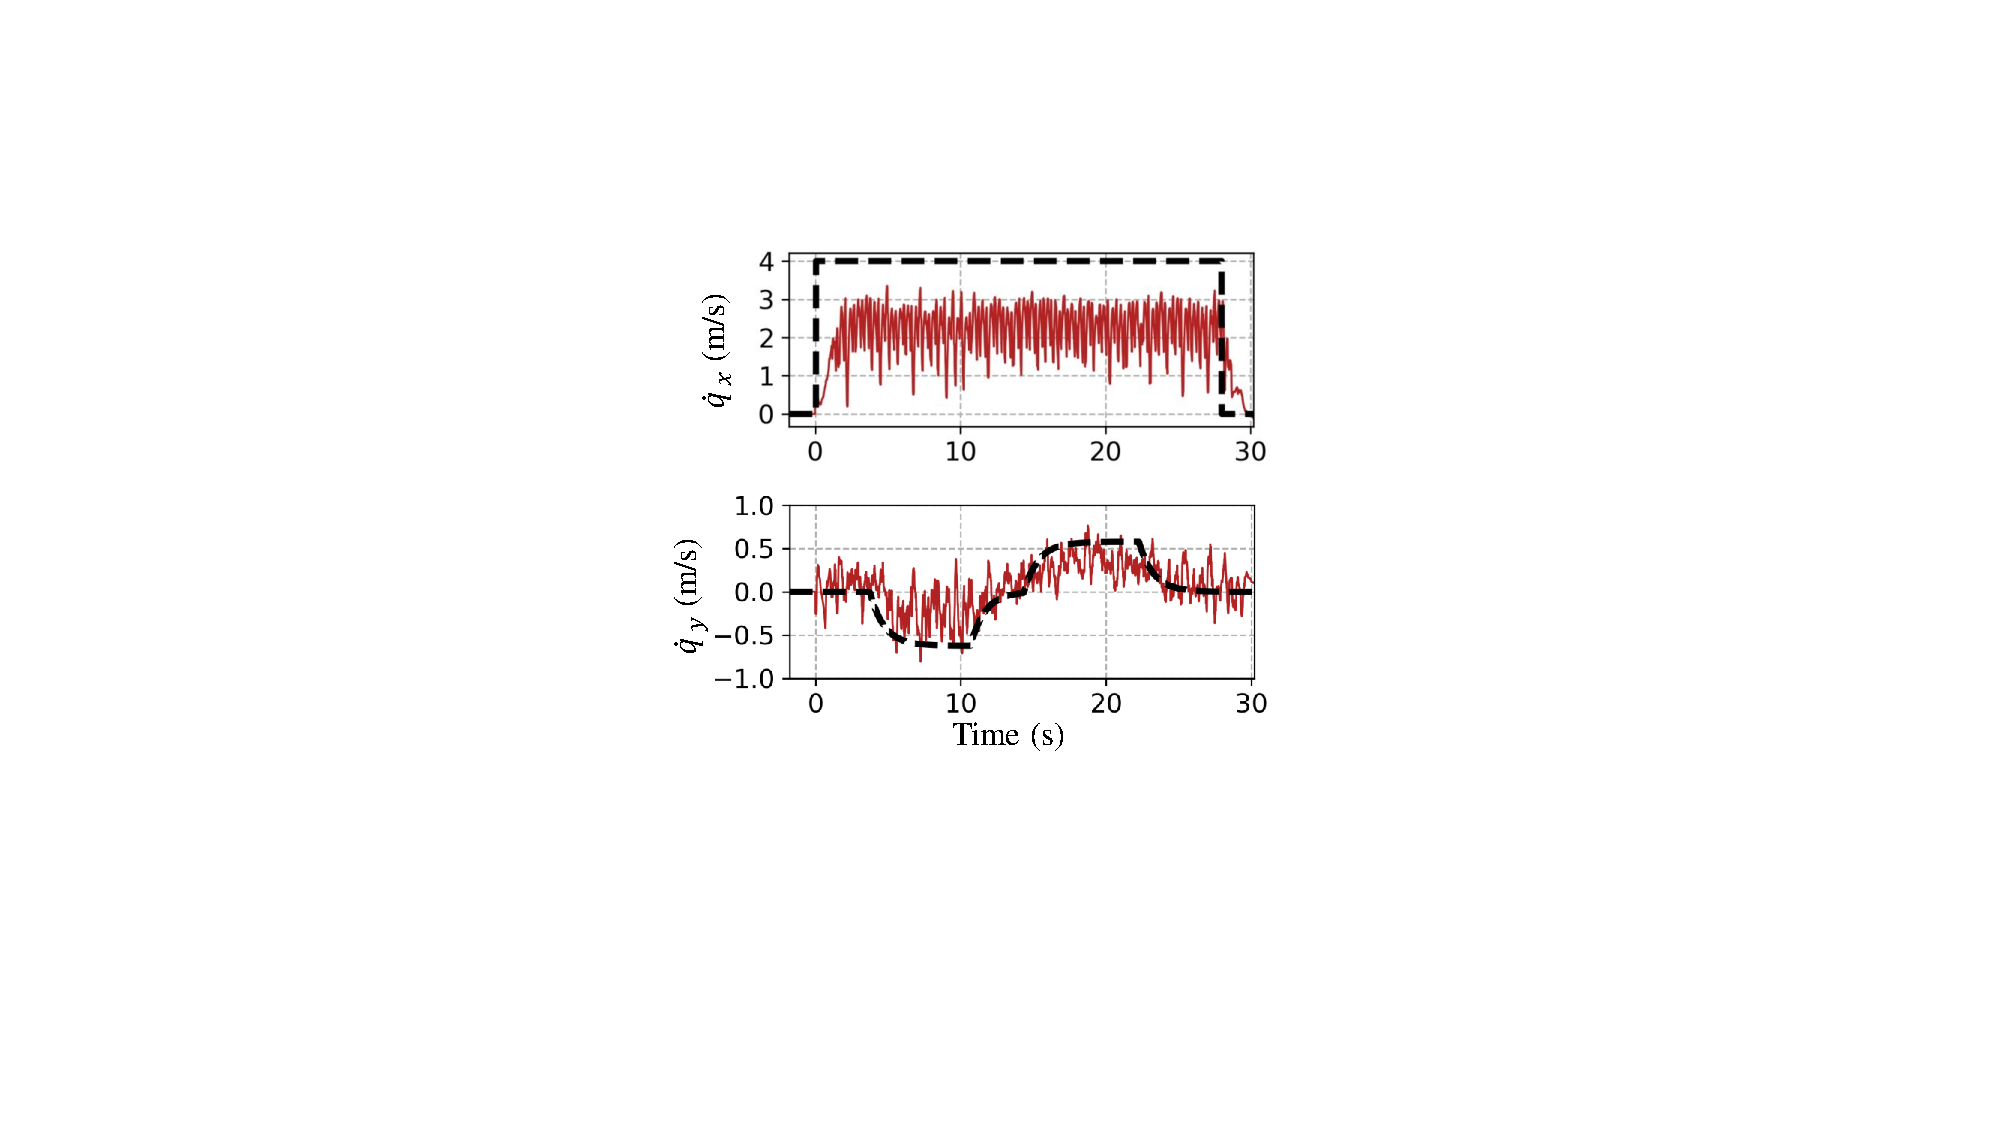
\includegraphics[width=\linewidth]{figures/run_variablevy.pdf}
  \caption{Tracking variable lateral velocity during running}
  \label{subfig:run_variablevy}
\end{subfigure}
\begin{subfigure}{0.375\linewidth}
  \centering
  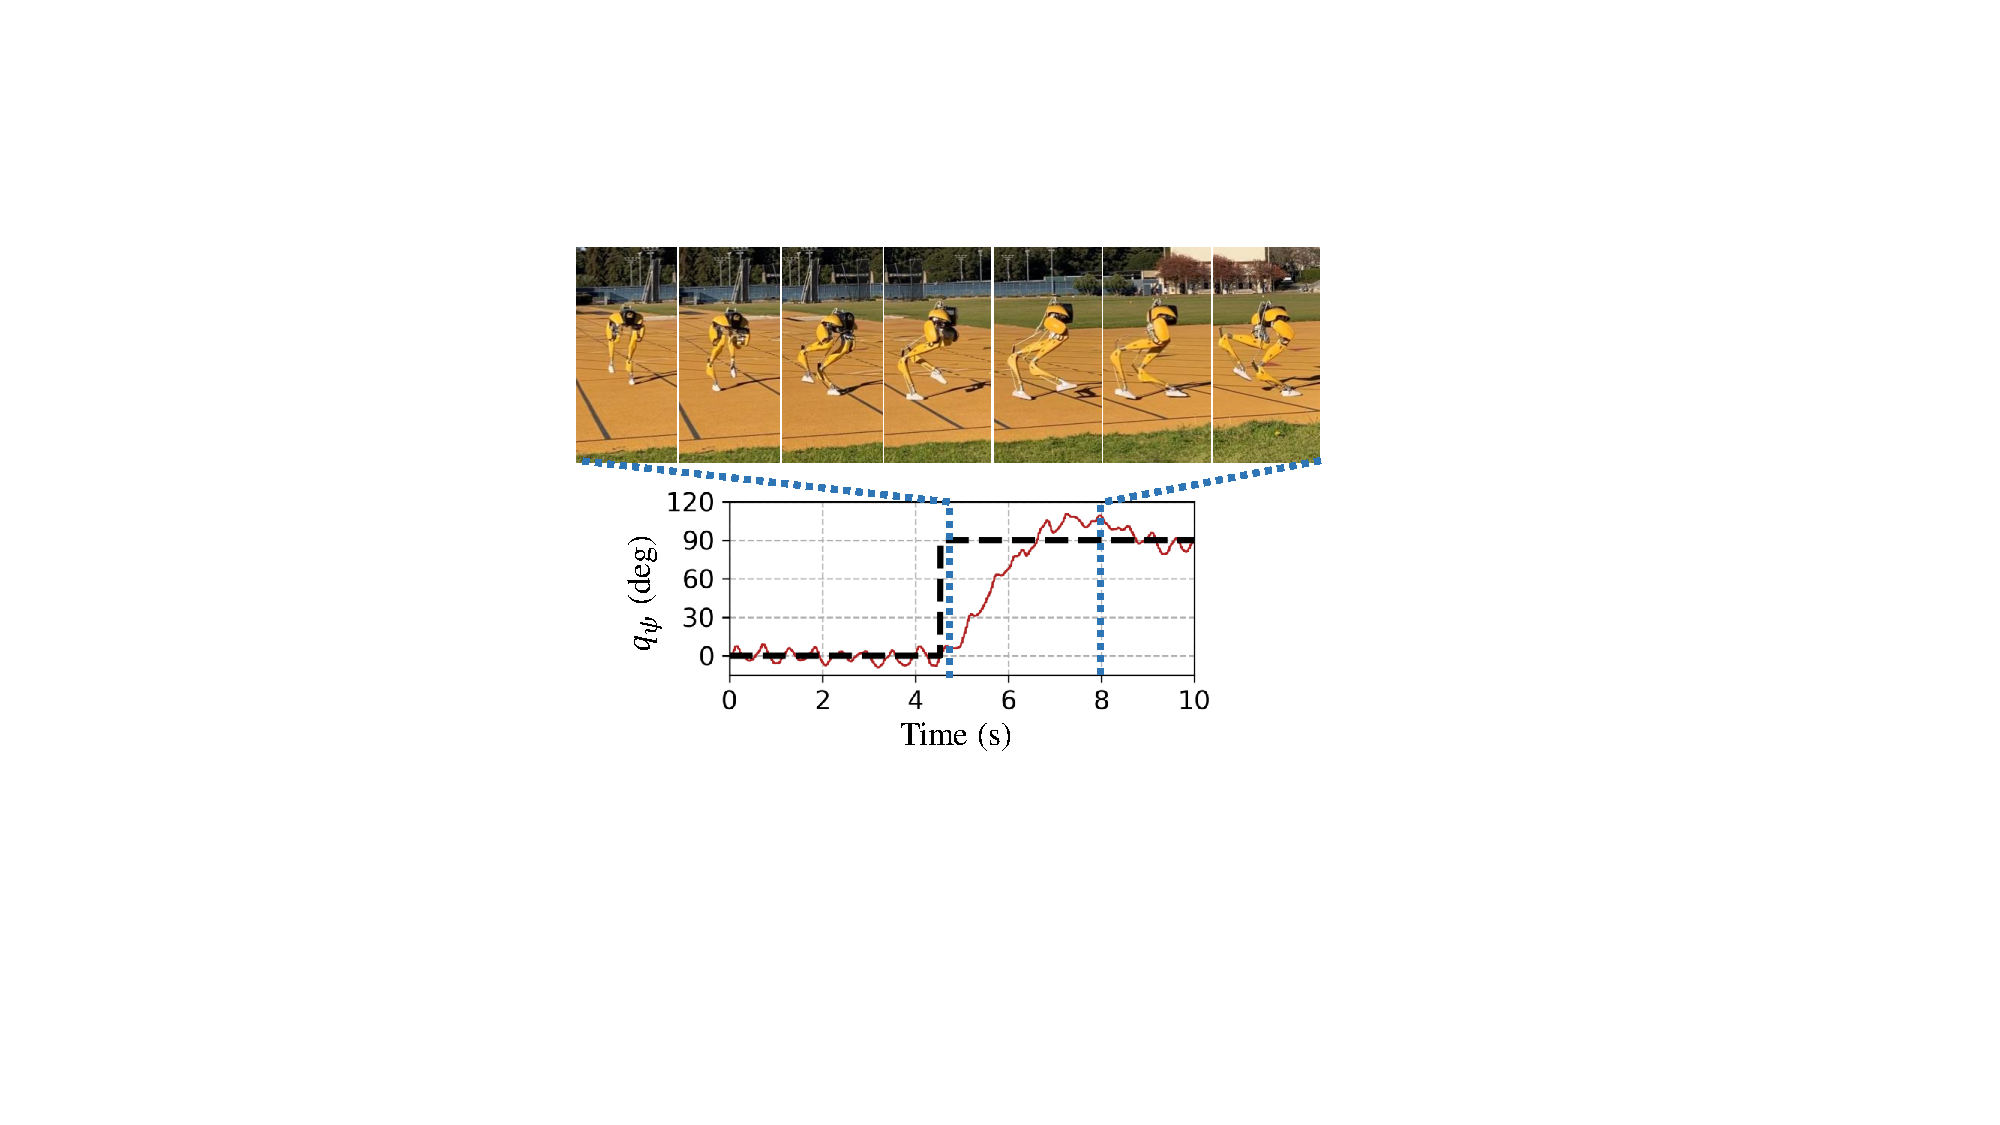
\includegraphics[width=\linewidth]{figures/run_sharpturn.pdf}
  \caption{Sharp turn during running. This scenario (tracking nonsmooth turning angle) is not specifically trained.}
  \label{subfig:run_sharpturn}
\end{subfigure}
\caption{Real-world experiments on tracking variable commands while running using the same control policy that completed the 400m-dash in Fig.~\ref{fig:400run}. Using the versatile policy, the robot is able to track varying sagittal velocity $\dot{q}_x$ (Fig.~\ref{subfig:run_variablevx}) and lateral velocity $\dot{q}_y$ (Fig.~\ref{subfig:run_variablevy}). Furthermore, the robot is able to perform a sharp turn while running, as demonstrated in Fig.~\ref{subfig:run_sharpturn}. The robot can turn to 90 degrees within 2 seconds, using 5 steps, as recorded in the logs and corresponding snapshots in Fig.~\ref{subfig:run_sharpturn}. Notably, the robot is not specifically trained for this sharp-turn scenario during training. These experiments are also recorded in Vid. 4 in Table~\ref{tab:video_list}.}
\label{fig:run_variable_cmd}
\end{figure*}




\subsection{Running Experiments}
We now evaluate the versatile running policies developed using the proposed methods in the real world. 
Three specific running policies were obtained: (1) a \emph{general policy} trained on flat ground; (2) a \emph{100-meter-dash finetuned policy}, trained after the convergence of the general policy with a focus on completing a 100-meter dash. This policy incorporated an additional termination condition to end the episode earlier if the robot could not complete the 100-meter dash within 25 seconds; (3) an \emph{uneven-terrain policy}, developed after the convergence of the general policy, integrated with extra terrain randomization as listed in Table~\ref{tab:randomization}.
All the policies have been trained with a variety of running and turning speeds as listed in Table~\ref{tab:command} and transition to and from a standing skill.
As we will see, using the obtained bipedal running policies, we achieved 400-meter dash within 2 min 34 s, 100-meter dash within 27.06 s, running inclines up to $10^\circ$, and more. 

\begin{figure*}[t]
\centering
\begin{subfigure}{\linewidth}
  \centering
  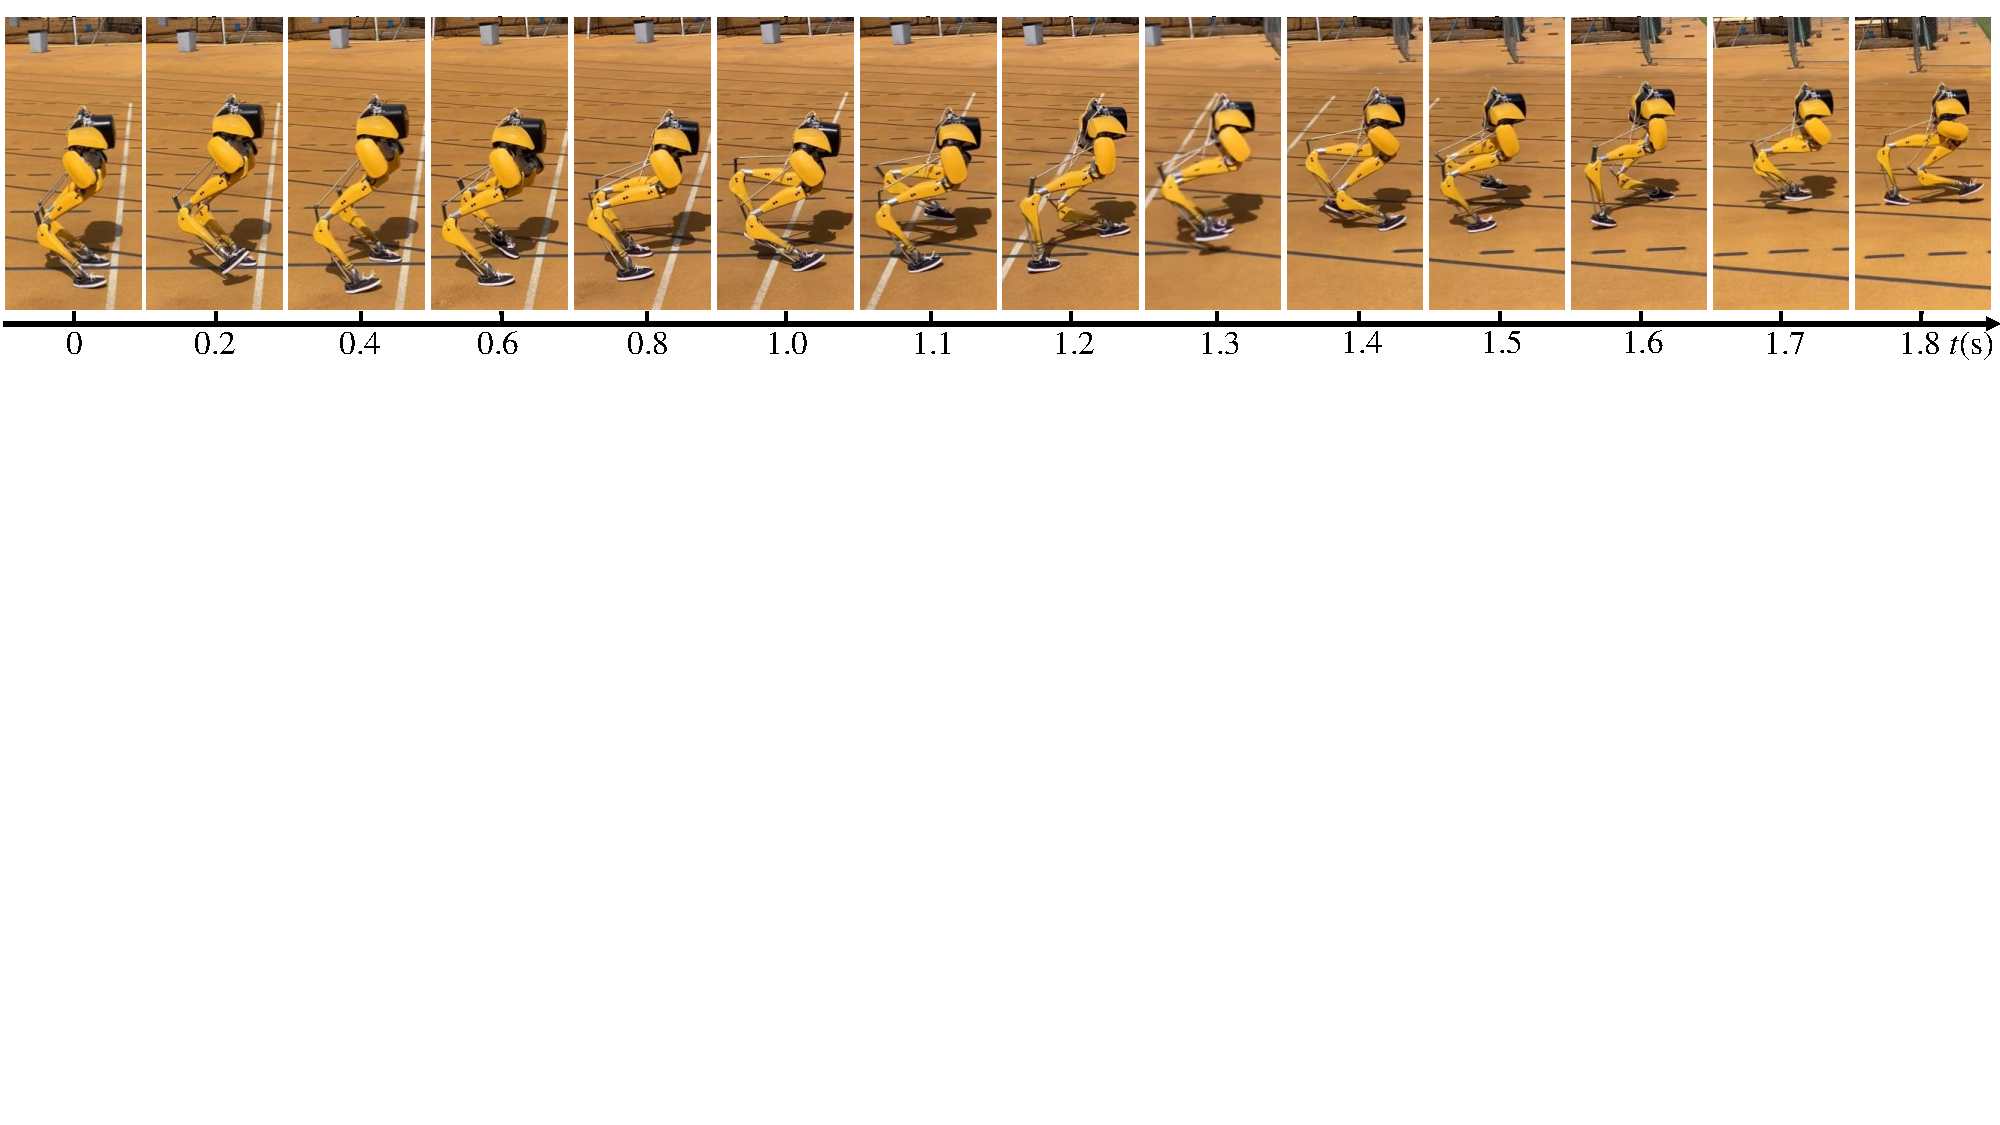
\includegraphics[width=\linewidth]{figures/run_100_init.pdf}
  \caption{Snapshot of the robot performing transition from standing to running in 100-meter dash, with timestamps indicating the corresponding frames}
  \label{subfig:run_100_init}
\end{subfigure}
\begin{subfigure}{\linewidth}
  \centering
  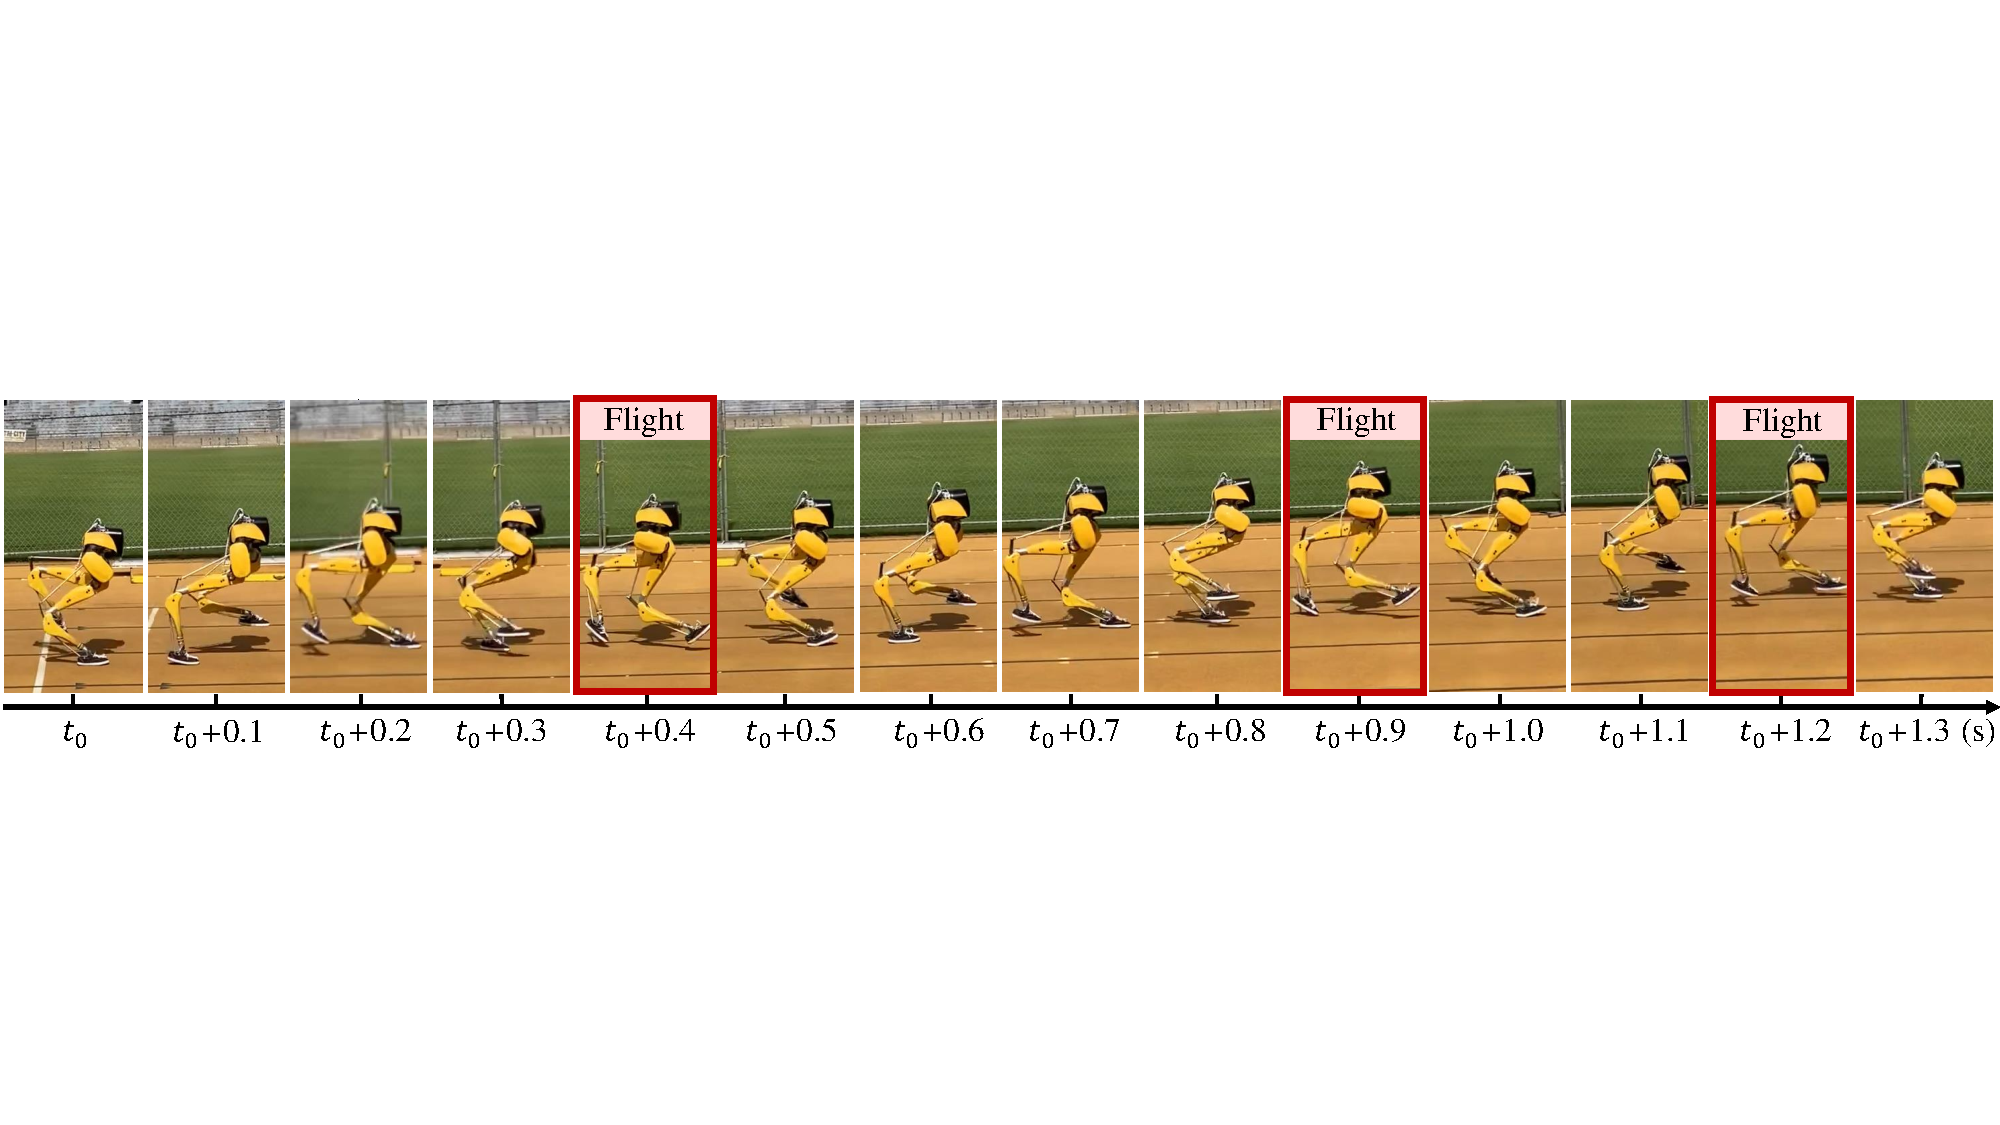
\includegraphics[width=\linewidth]{figures/run_100_curise.pdf}
  \caption{Snapshot of the robot running during 100-meter dash, with timestamps indicating the corresponding frames}
  \label{subfig:run_100_cruise}
\end{subfigure}  
\begin{subfigure}{\linewidth}
  \centering
  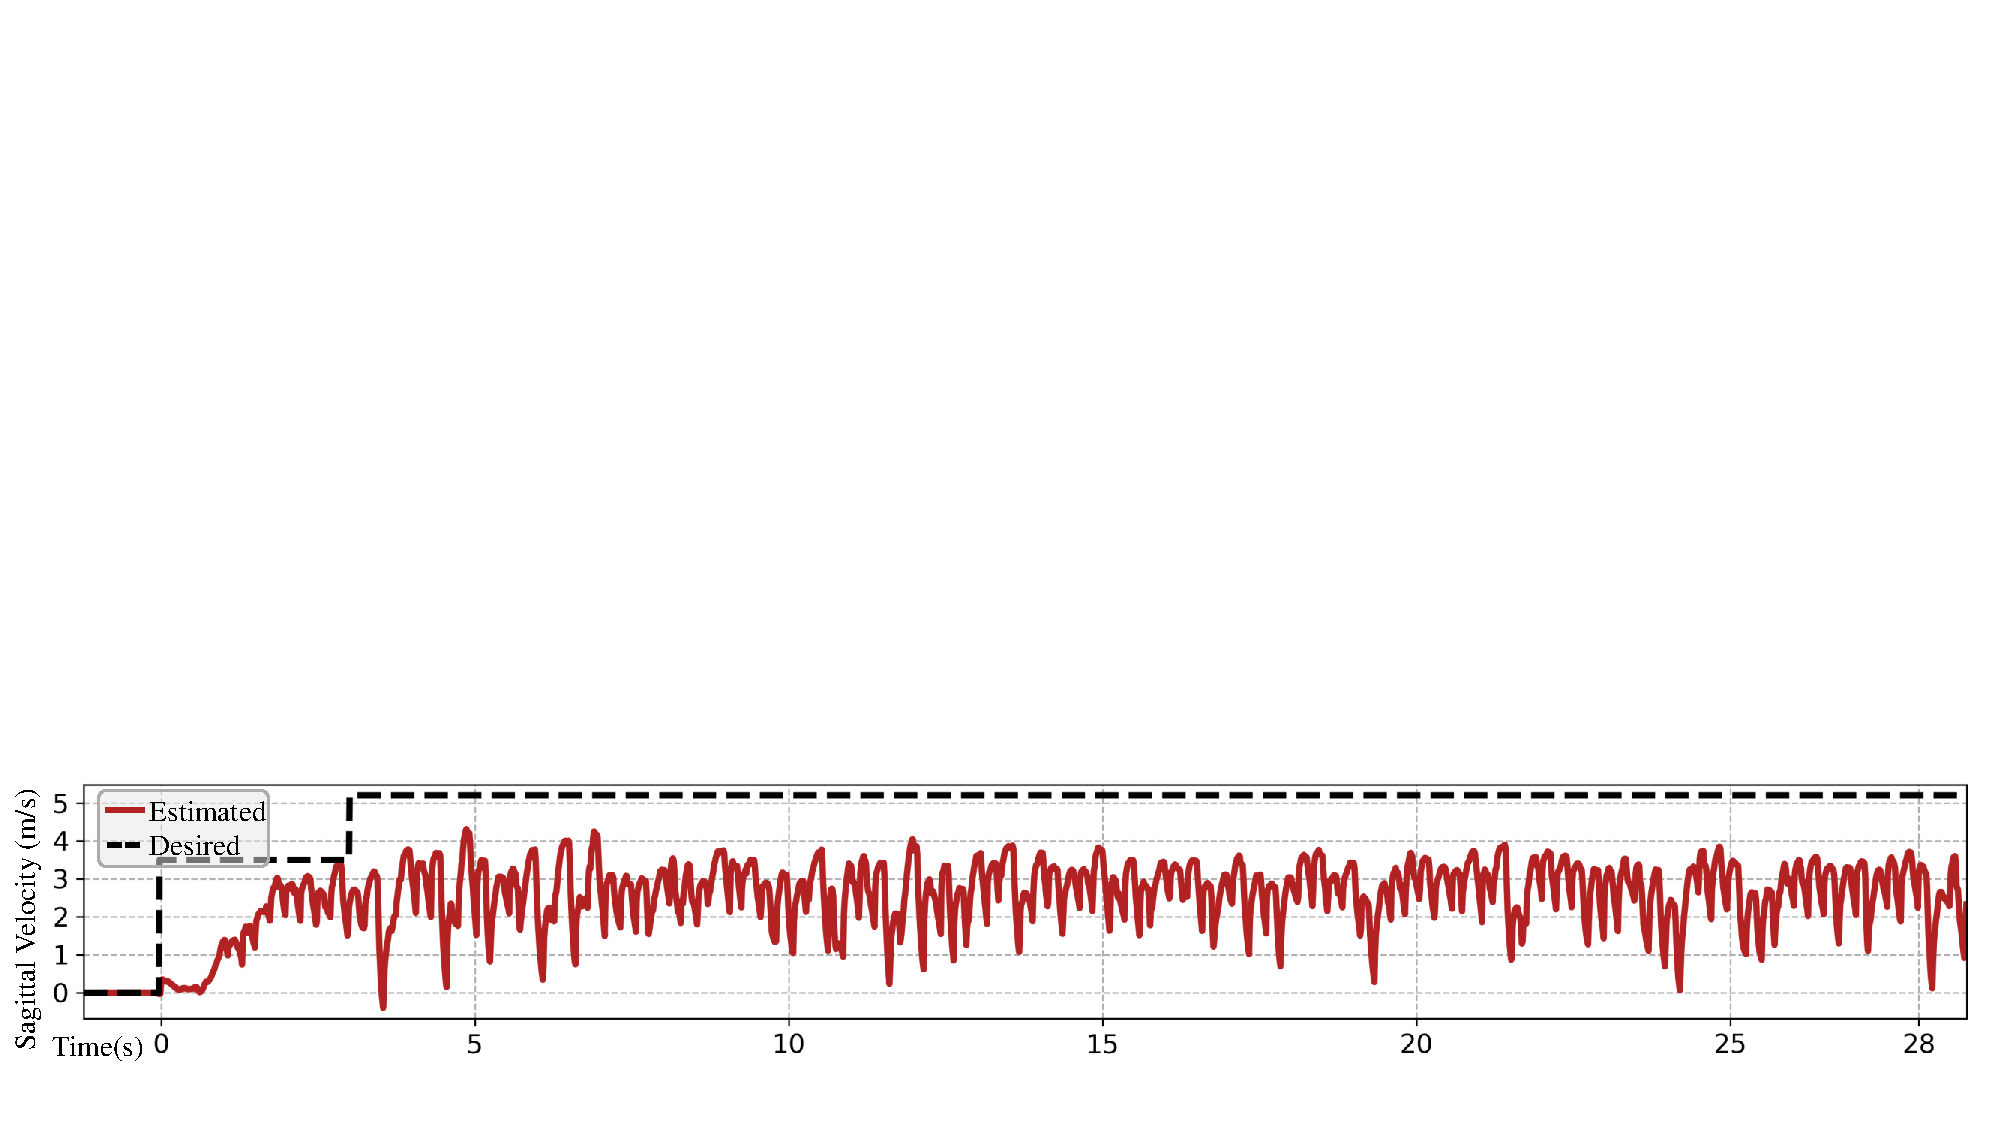
\includegraphics[width=\linewidth]{figures/run_100_log.pdf}
  \caption{Recorded sagittal velocity $\dot{q}_x$ in the 100-meter dash}
  \label{subfig:run_100_log}
\end{subfigure}  
\caption{Using the finetuned running policy, Cassie finishes the 100-meter dash with a fast running gait. Fig.~\ref{subfig:run_100_init} shows that the robot is able to transit from stationary stance to a rapid running gait, accelerating from 0 m/s to 3 m/s within 2 seconds with aggressive maneuvers. During the cruise phase shown in Fig.~\ref{subfig:run_100_cruise}, the robot maintains a fast yet stable running gait. The corresponding commanded and \emph{estimated} sagittal velocity $\dot{q}_x$ is recorded in Fig.~\ref{subfig:run_100_log}. The robot finished this dash within 28 seconds, with an average speed of 3.57 m/s.}
\label{fig:100run}
\end{figure*}




\subsubsection{Running a 400-meter Dash}
We first evaluate the general running policy to complete a 400-meter dash on a standard outdoor running track, as demonstrated in Fig.~\ref{fig:400run}.
Throughout this test, the robot was commanded to run at a consistent 3.5 m/s while responding to varying turning commands, given by a human operator to navigate the track. 
As shown in Fig.~\ref{subfig:run_400_snapshot} and the accompanying Vid. 2 in Table~\ref{tab:video_list}, the policy is able to smoothly transition from a standing position to a running gait (Fig.~\ref{subfig:run_400_snapshot}\circled{1}). 
The robot managed to accelerate to an average \emph{estimated} running speed of 2.15 m/s\footnote{We note that there is a nontrivial state estimation error on the sagittal velocity when the robot is running at a high speed. The average speed of finishing 400 meter in 154 seconds is 2.6 m/s while the estimated average speed is 2.15 m/s. Such an error is more obvious in the 100-meter dash discussed later. Therefore, we emphasize the logs are estimated values and not true values. We further elaborate this in Appendix~\ref{appendix:estimaion_error}.}, reaching a peak estimated speed of 3.54 m/s, as recorded in Fig.~\ref{subfig:run_400_log}.
The policy successfully maintained the desired speed consistently throughout the entire 400-meter run while accurately adhering to the varying turning commands. 
The average tracking error (MAE) in the turning angle $q_{\psi}$ observed in Fig.~\ref{subfig:run_400_log} is 5.95 degrees.
Throughout the 400m-dash, substantial flight phases were evident, as shown in Fig.~\ref{subfig:run_400_snapshot}\circled{2}-\circled{4}, despite the variable running speeds and turning angles. 
This consistent flight phase distinguishes our running gaits from a fast walking gait and presents significantly more challenges in control. 
However, the controller managed to sustain such a dynamic running gait stably over a significant duration (154 seconds).

Furthermore, during the 400-meter dash, although some lateral drift was detected, as shown in Fig.~\ref{subfig:run_400_log}, the robot can keep an average lateral velocity of 0.05 m/s. 
While the average lateral speed is relatively negligible, the robot did exhibit moments of having higher lateral speeds, exceeding 1 m/s at times, possibly due to irregular contact in the real-world environment. 
However, the policy's training in lateral running skills allowed the robot to correct these deviations, demonstrating the policy's robustness in maintaining stability even in the face of such unexpected lateral movements.

Cassie, controlled by the proposed running policy, successfully finished the 400-meter dash in \emph{2 minutes and 34 seconds}, and was able to transit to a standing pose afterward, as recorded in the video. 
This is a novel capacity of running a full 400-meter lap by a human-sized bipedal robot. 





\subsubsection{Tracking Varying Commands while Running}
Using the same versatile policy, the robot is also able to reliably track varying commands, such as sagittal velocity $\dot{q}_x$ shown in Fig.~\ref{subfig:run_variablevx} and lateral velocity $\dot{q}_y$ recorded in Fig.~\ref{subfig:run_variablevy}, while running fast. The corresponding experiments are recorded in Vid. 4 in Table~\ref{tab:video_list}. 
Note that only one dimension of the command is changing during each of the tests conducted in Figs.~\ref{subfig:run_400_log} (turning yaw $q_{\psi}$),~\ref{subfig:run_variablevx} (sagittal velocity),~\ref{subfig:run_variablevy} (lateral velocity). 
By comparing with the recorded logs among these tests, we observed that the command changing in one dimension will not affect the control performance on tracking a constant in other dimensions. 
This indicates that the dimensions on $\dot{q}_x$, $\dot{q}_y$, and $q_{\psi}$ are \emph{decoupled}, which is intriguing as this is realized in fast running control of a highly-nonlinear bipedal robot in the real world.











We further conduct a sharp turning test where the robot is given a step change of the yaw command, from 0 directly to 90 degrees, as recorded in Fig.~\ref{subfig:run_sharpturn}. 
The robot can respond to such a step command and finish a 90-degree sharp turn within 5 steps in 2 seconds, using a natural running gait shown in Fig.~\ref{subfig:run_sharpturn}. 
Remarkably, the robot is not specifically trained for this sharp-turn scenario, as only smooth turning yaw angle command whose changing rate is bounded to 30 deg/s is given during training, as listed in Table~\ref{tab:command}. 
The versatile policy can generalize the learned various turning tasks and direct transfer to accomplish such a sharp-turn test. 
This further highlights the advantage of obtaining a versatile policy as previous work like \cite{yu2022dynamic} requires training a separated policy to perform similar sharp-turn while walking. 







\begin{table}[t]
\centering
\caption{Record of the completion time of 100-meter dash in three trials in the real world.}
\label{tab:100run}
\begin{tabular}{cc}
\hline
Trial & Completion Time (s) \\ \hline
1     & 27.06               \\
2     & 27.99               \\
3     & 28.28               \\ \hline
\end{tabular}
\end{table}





\subsubsection{Running a 100-meter Dash}
We now assess the running policy fine-tuned for the 100-meter dash, documented in Fig.~\ref{fig:100run}. We conducted the test 3 times, results of which are detailed in Table~\ref{tab:100run} and available in Vid. 1 and Vid. 4 in Table~\ref{tab:video_list}.
With the deployment of the proposed running policy, the robot accomplished the 100-meter dash with around $28$ seconds, achieving a fastest run time of 27.06 seconds. 
As depicted in Fig.~\ref{subfig:run_100_init}, the robot quickly transitioned from a stationary standing pose to a fast running gait within 1.8 seconds, using the transition maneuvers we commonly observed in human running athletes. 
During the cruising phase (Fig.~\ref{subfig:run_100_cruise}), the robot maintained a rapid running gait and reached a peak estimated speed of 4.2 m/s, showing notable flight phases, as the data recorded in Fig.~\ref{subfig:run_100_log}. 



\begin{figure*}[t]
\centering
\begin{subfigure}{0.535\linewidth}
  \centering
  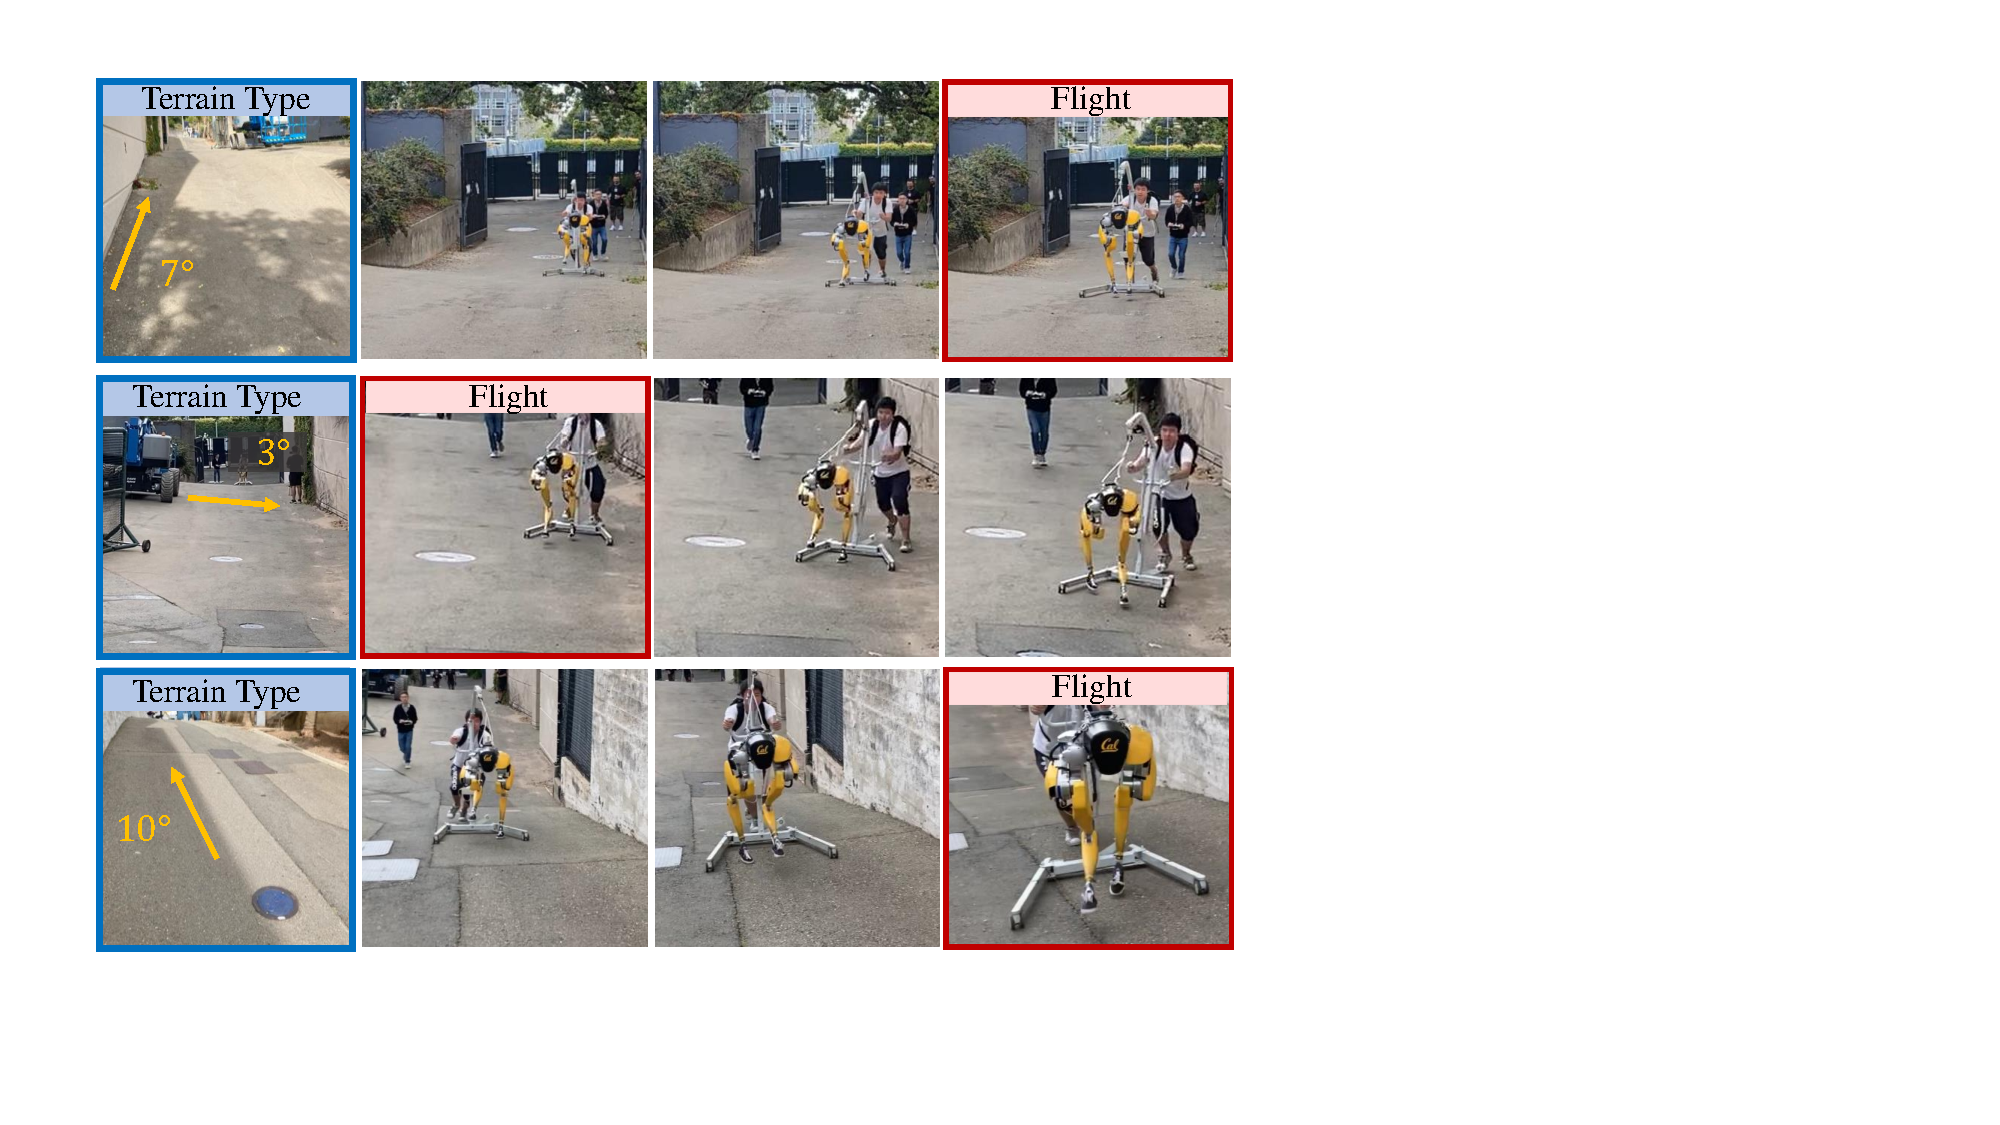
\includegraphics[width=\linewidth]{figures/run_terrain_snapshot.pdf}
  \caption{Snapshot of the robot running on varying terrains}
  \label{subfig:run_terrain_snapshot}
\end{subfigure}
\begin{subfigure}{0.41\linewidth}
  \centering
  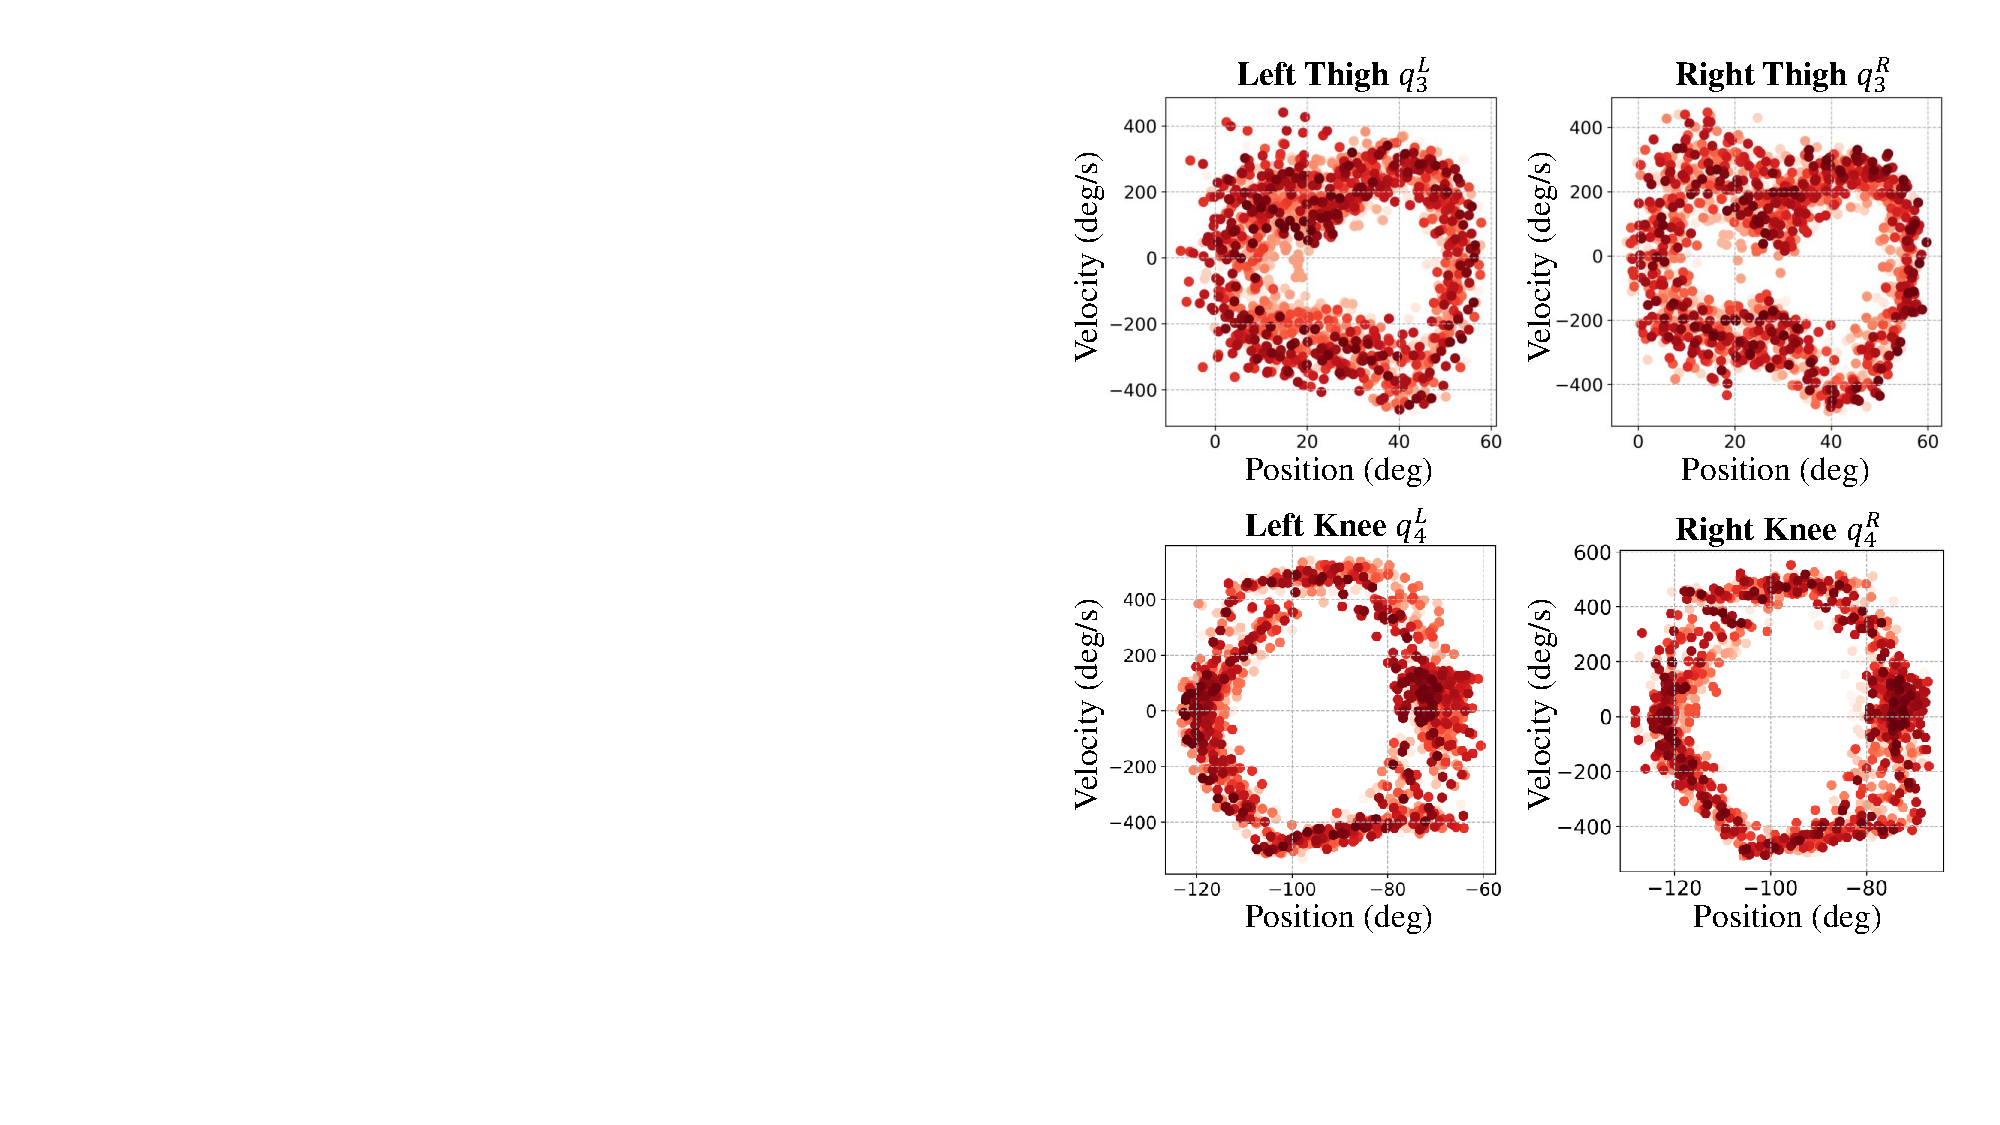
\includegraphics[width=\linewidth]{figures/run_terrain_phaseplot.pdf}
  \caption{Recorded phase plots of thigh and knee joints}
  \label{subfig:run_terrain_phaseplot}
\end{subfigure}  
\caption{The robot runs over various terrains without any prior knowledge of the terrain specifics or elevation estimates. Fig.~\ref{subfig:run_terrain_snapshot} records the robot running on different types of terrains with different slopes, starting from 7$^\circ$ incline in the sagittal direction, followed by a 3$^\circ$ slope laterally, then a 10$^\circ$ sagittal incline, and finally transitioning to flat ground. The left-most column of the figure showcases these different terrain types. Despite the varying terrain, the robot consistently adapts and maintains a stable running gait with noticeable flight phases, as shown in the right columns of the figure. Fig.~\ref{subfig:run_terrain_phaseplot} records the corresponding phase plots of the robot thigh and knee joints ($q^{L/R}_{3,4}$ versus $\dot{q}^{L/R}_{3,4}$, which play dominant roles in locomotion control), showing converged limit cycles.}    
\label{fig:run_terrain}
\end{figure*}



\begin{figure*}[t]
\centering
\begin{subfigure}{\linewidth}
  \centering
  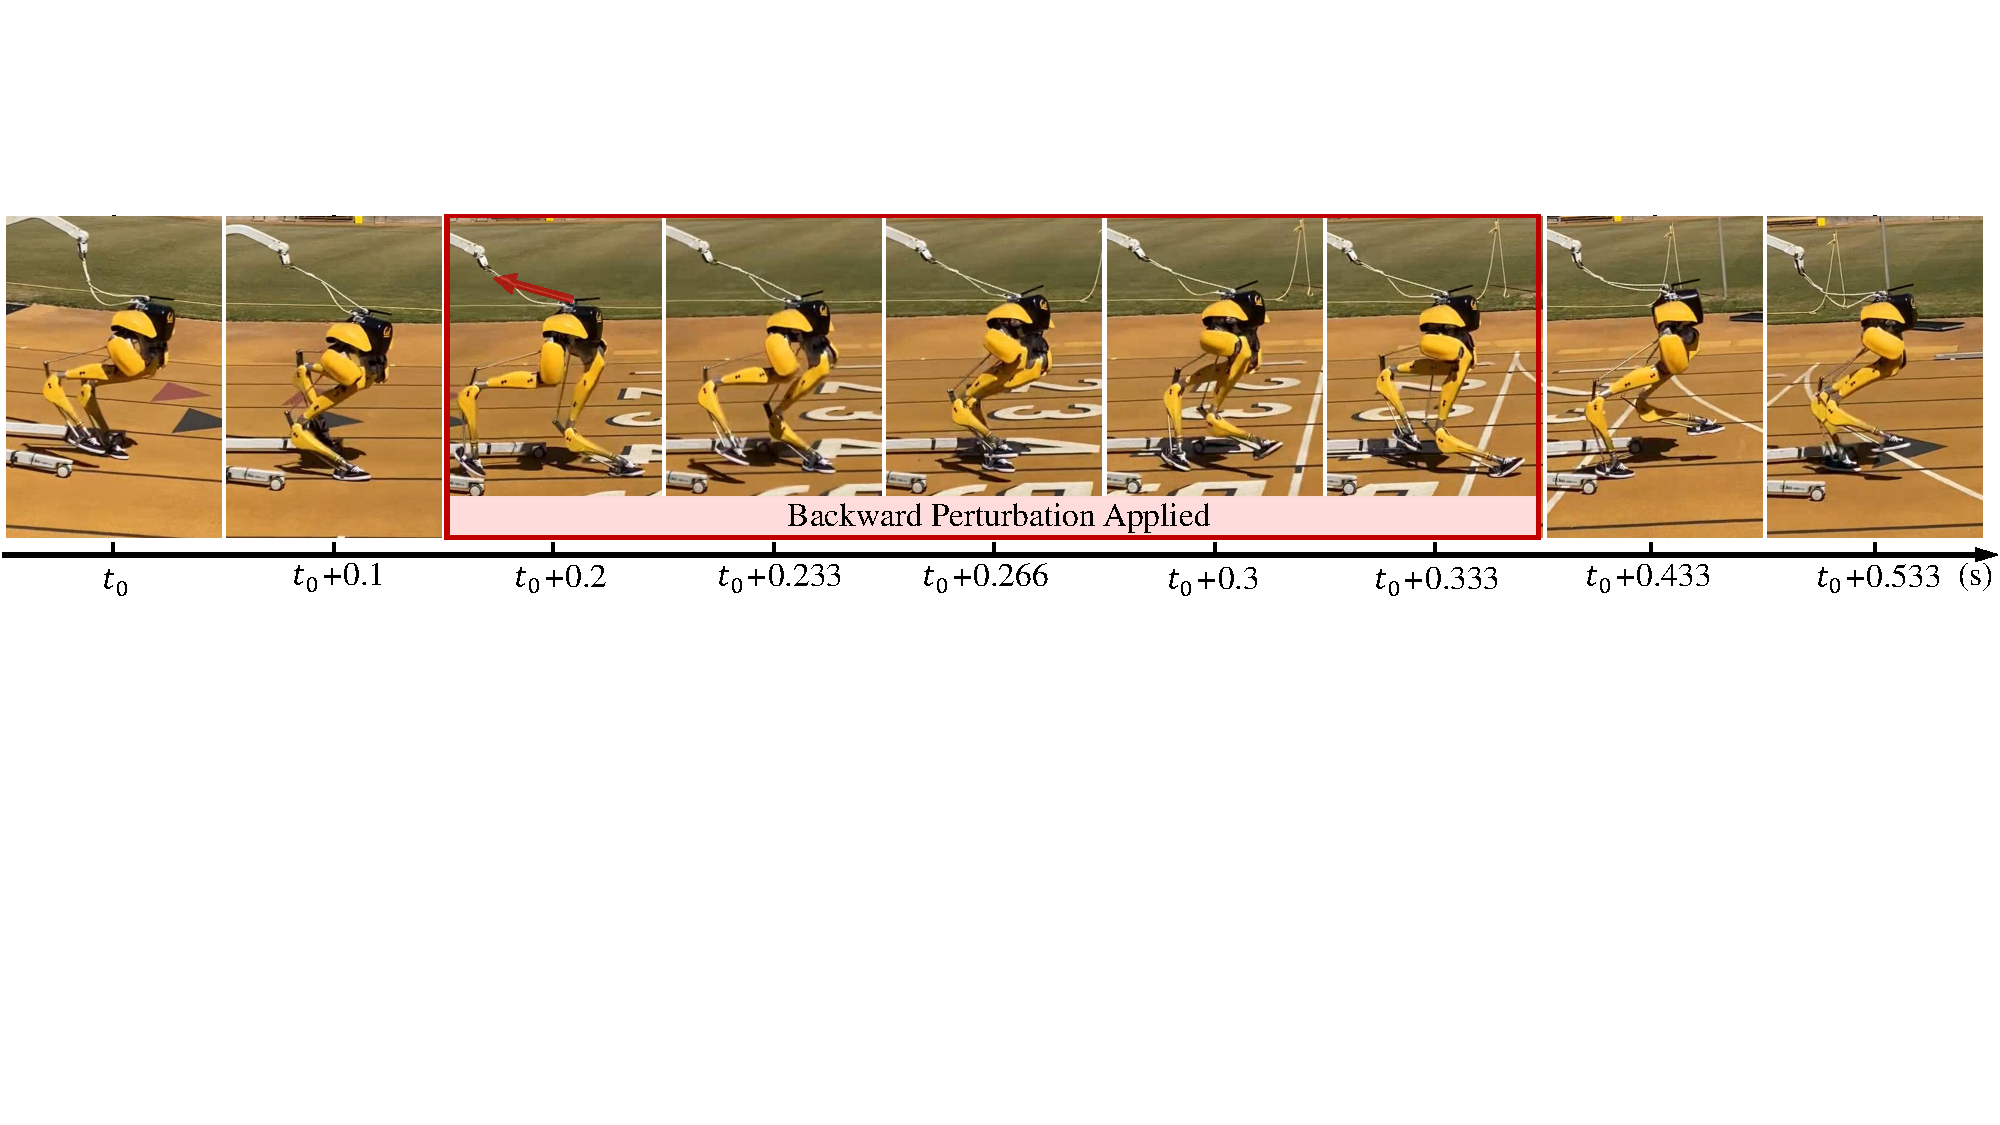
\includegraphics[width=\linewidth]{figures/running_perturb.pdf}
  \caption{The robot covers from a backward perturbation during running}
  \label{subfig:run_perturb}
\end{subfigure}
\begin{subfigure}{\linewidth}
  \centering
  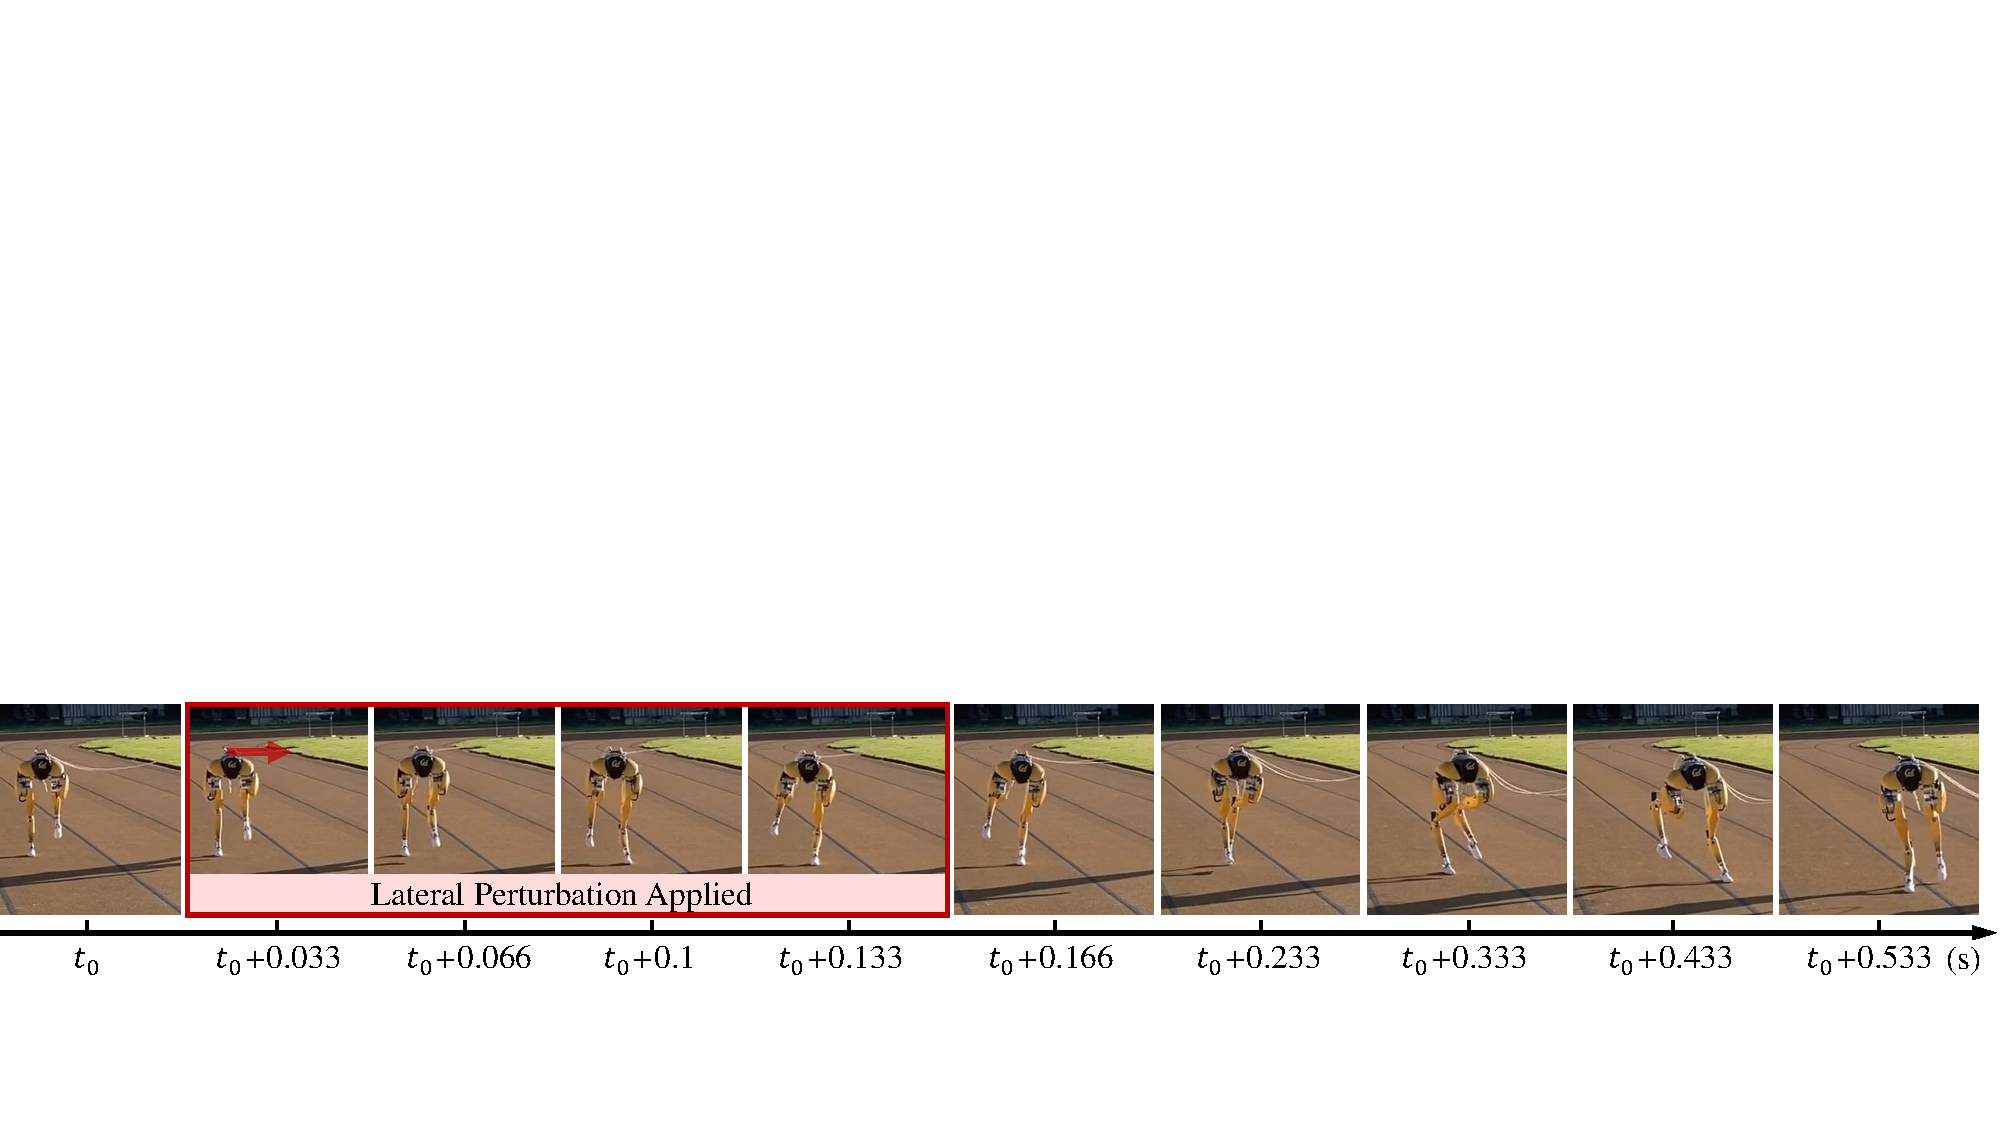
\includegraphics[width=\linewidth]{figures/running_lateral_perturb.pdf}
  \caption{The robot recovers from a lateral perturbation during running}
  \label{subfig:run_lateral_perturb}
\end{subfigure}  
\caption{Snapshot that captures the moment when the robot, while running a 100-meter dash with a fast speed, is unexpectedly perturbed, demonstrating the robustness of the versatile running policy we developed. The frames are aligned with the corresponding timestamps. The robot experiences a sudden decrease in speed and begins to lean laterally along with a significant drift in its base yaw angle, due to being pulled backward by the safety cord. Despite these deviations from its nominal running trajectory, the robustness of the policy, which is enhanced by training with extensive dynamics randomization and versatile tasks (including slower-speed running with lateral and turning commands), enables the robot to maintain stability and correct itself back.}
\label{fig:run_perturb}
\end{figure*}





\subsubsection{Running on Uneven Terrains (Trained)}
We proceed to examine the running policy fine-tuned for uneven terrains. 
As observed in Fig.~\ref{subfig:run_terrain_snapshot}, the robot controlled by the proposed running policy managed to effectively traverse terrains with different slopes, all without the need for explicit terrain height estimation or external sensors.
The terrain tests encompassed challenging variations, beginning with a $7^\circ$ inclined slope in the sagittal plane, followed by a $3^\circ$ slope in the lateral plane, a steeper $10^\circ$ inclined slope in the sagittal plane, and concluding with a flat ground. 
Despite these difficult terrains, the robot maintained a stable running gait, as indicated by the converged limit cycles of the robot's thigh and knee joints ($q^{L/R}_{3,4}$) showcased in Fig.~\ref{subfig:run_terrain_phaseplot} across these varied elevations.
The robot's ability to change its gait to adapt to different terrains is derived from its usage of the robot's input/output history, implicitly encapsulating information about contact events and positioning.
Notably, even while traversing these challenging terrains, the robot retained its flight phase, as showcased in Fig.~\ref{subfig:run_terrain_snapshot}, signifying its ability to maintain a running gait, avoiding a degradation to walking gaits that offer more support but reduced speed.
This is the first implementation of running (with flight phases) over large uneven terrains by a human-sized bipedal robot. 







\begin{figure*}[t]
\centering
\begin{subfigure}{0.495\linewidth}
  \centering
  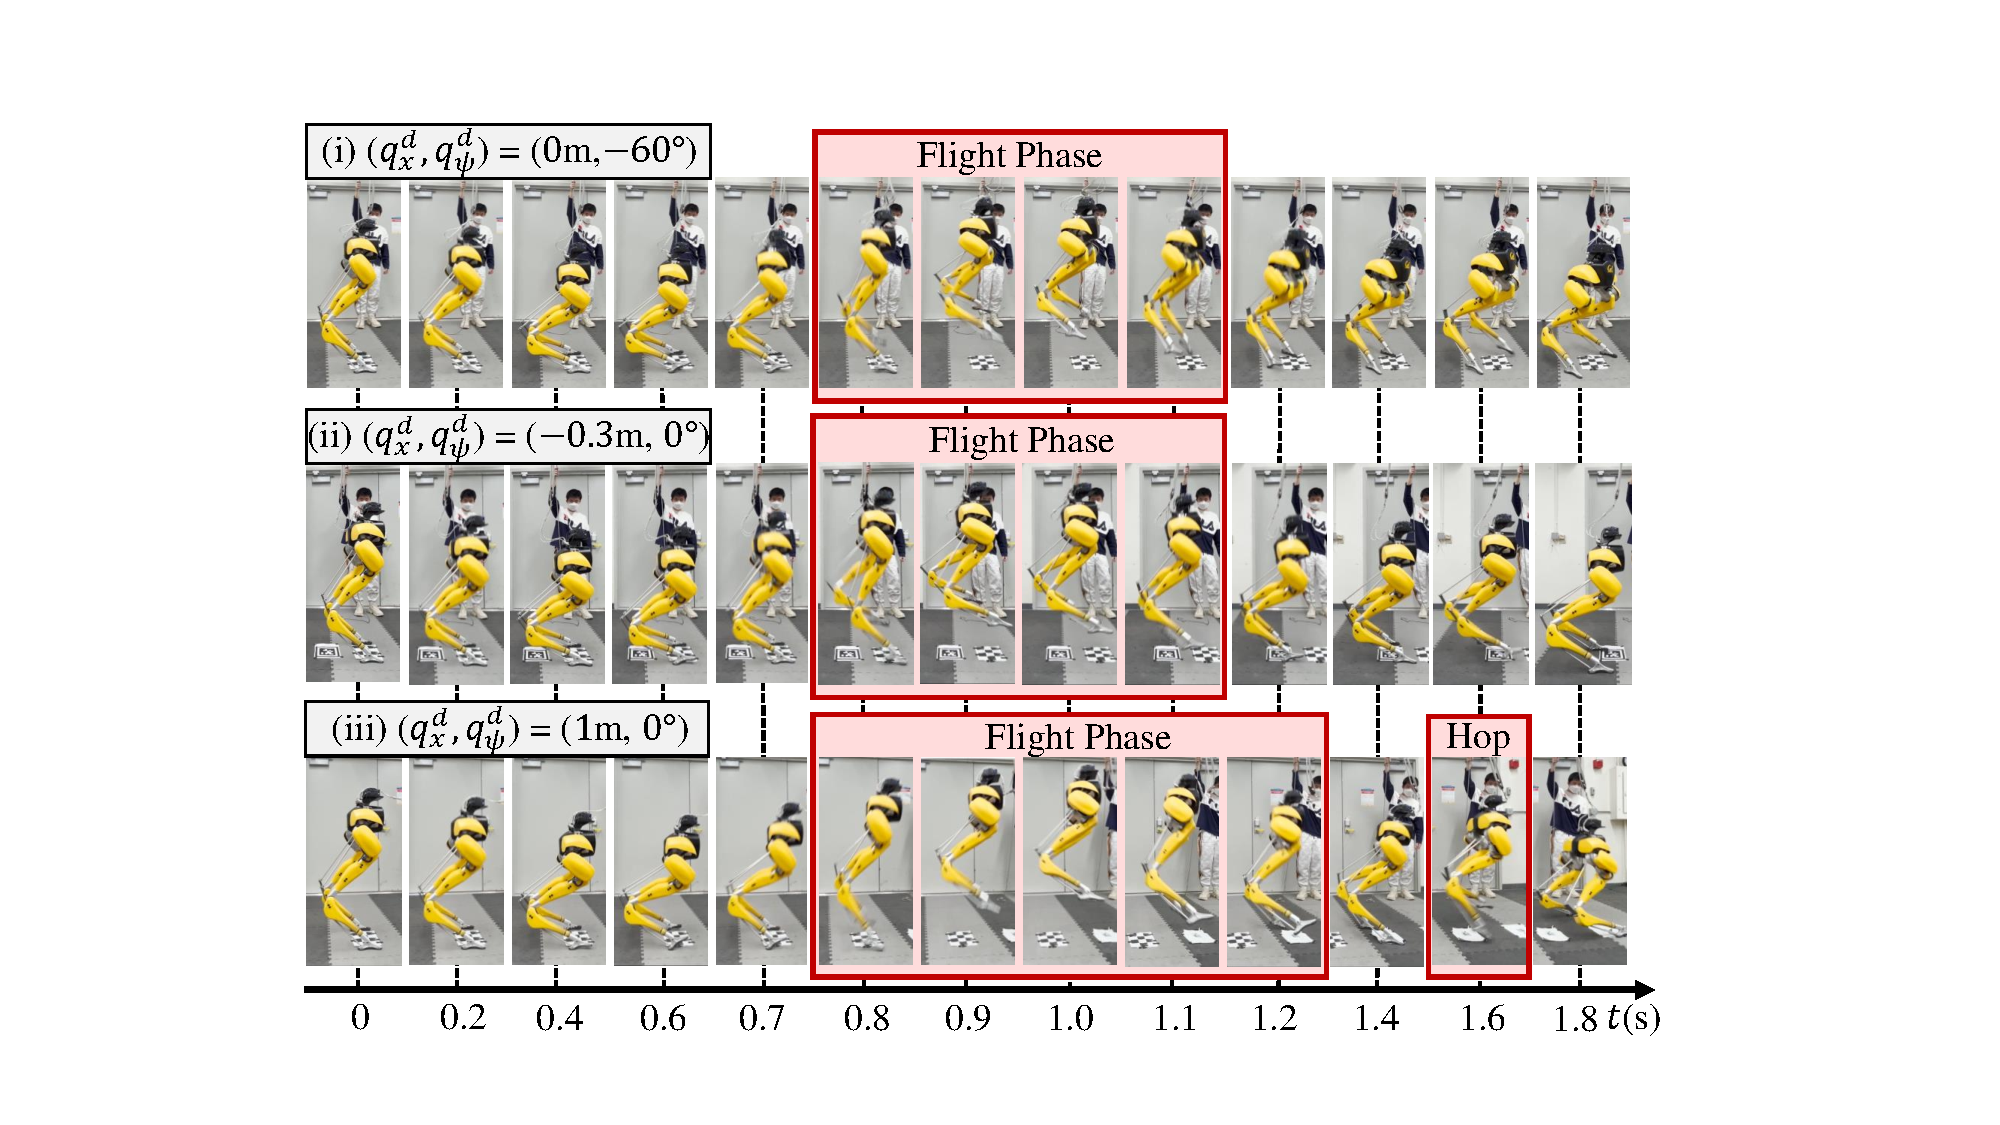
\includegraphics[width=\linewidth]{figures/flat_ground_snapshot.pdf}
  \caption{Different jumps using the flat-ground policy}
  \label{subfig:snapshot_flatx3}
\end{subfigure}
\begin{subfigure}{0.495\linewidth}
  \centering
  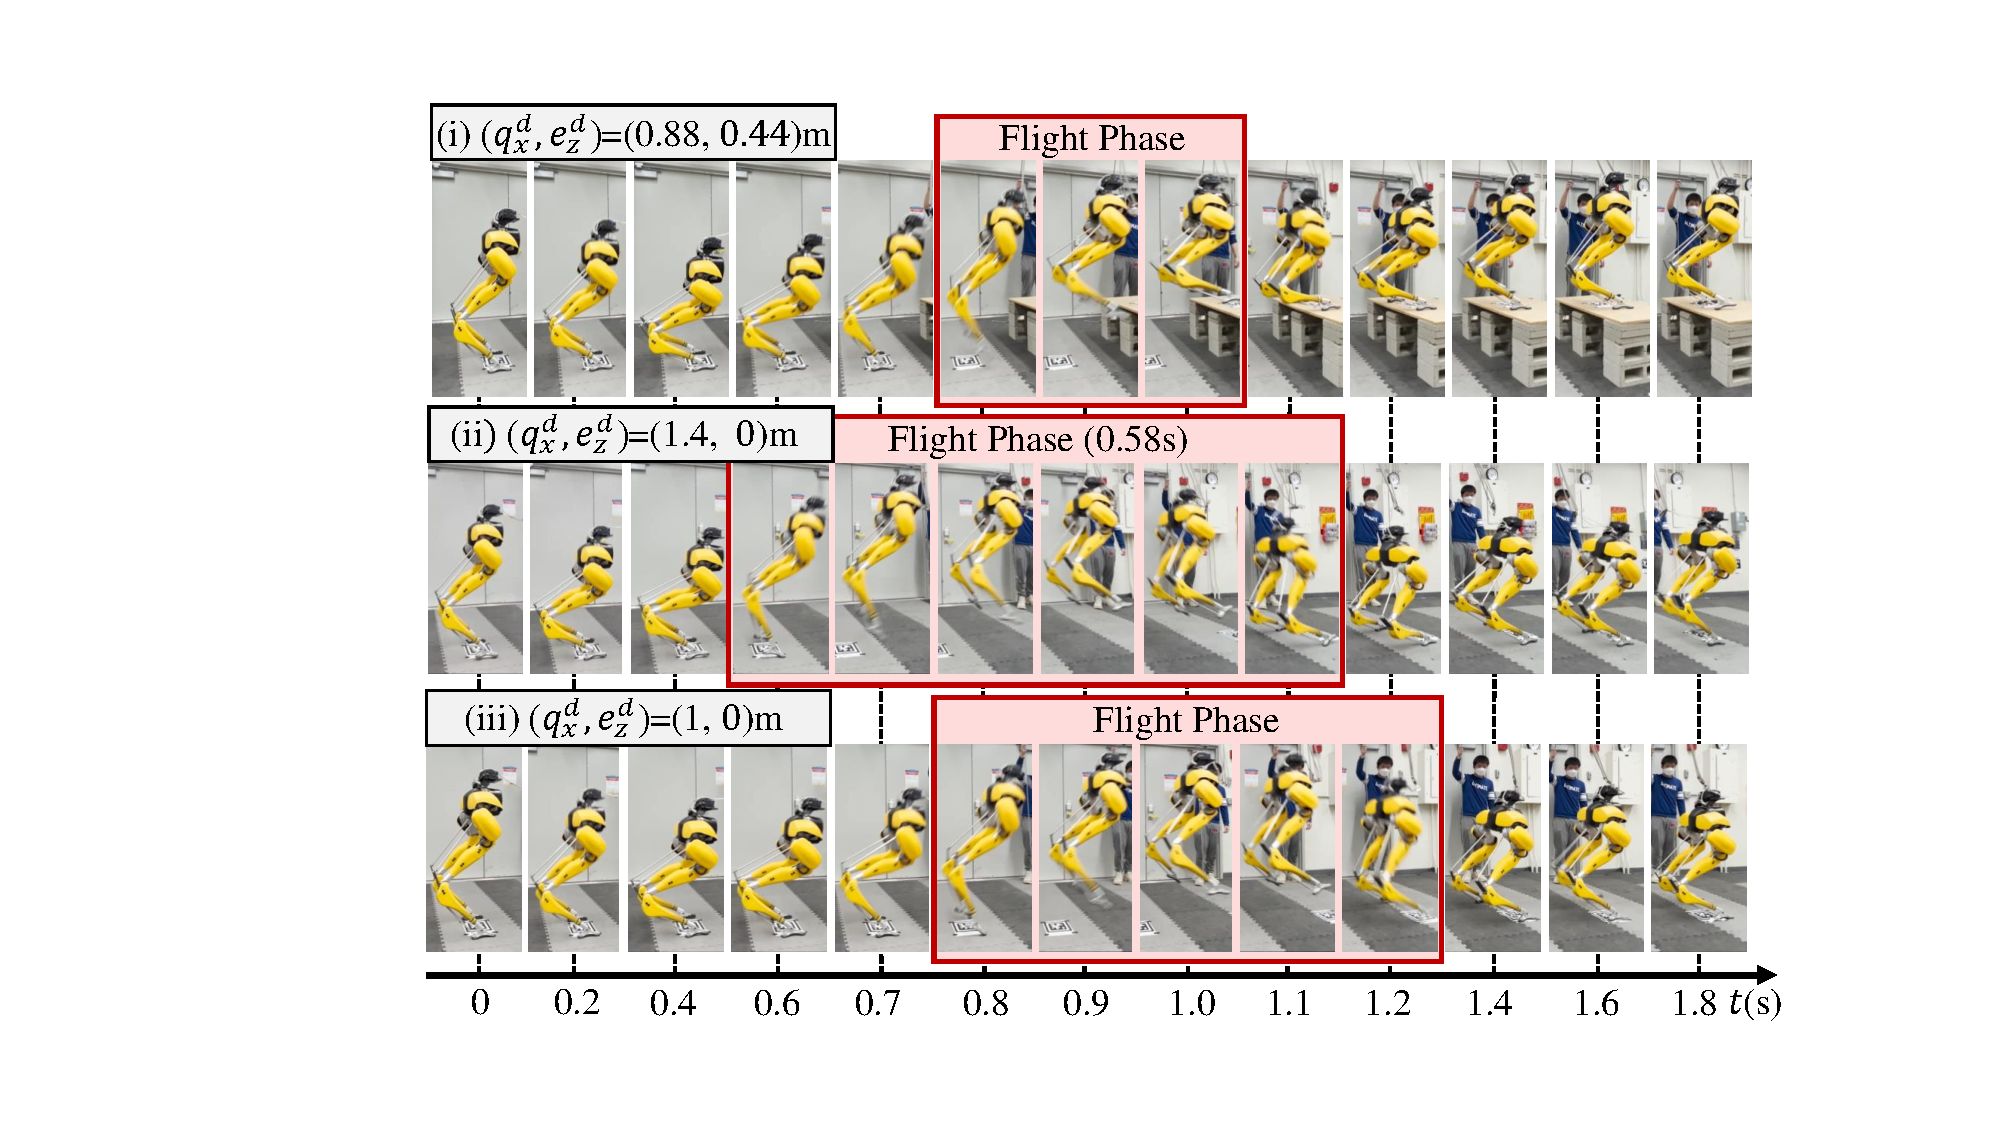
\includegraphics[width=\linewidth]{figures/discrete_terrain_snapshot.pdf}
  \caption{Different jumps using the discrete-terrain policy}
  \label{subfig:snapshot_tablex3}
\end{subfigure}
\caption{Snapshots of the bipedal robot Cassie performing various aggressive jumping maneuvers using two single versatile policies. Each frame is aligned with the corresponding timestamp, and paper tags in the figures represent the desired landing target. In Fig.~\ref{subfig:snapshot_flatx3}, using the \textit{flat-ground} policy, (i) the robot is able to perform in-place jump while turning, (ii) backward jump, and (iii) forward jump, and land accurately on the target (paper tag). During the 1-meter ahead jump, the robot interestingly performs an extra forward hop after its initial landing, reaching the target on this second attempt. This additional maneuver was not observed during simulations that utilized the robot's nominal model. In Fig.~\ref{subfig:snapshot_tablex3}, using the \textit{discrete-terrain} policy, (iii) the robot is also able to perform 1-meter forward jump. Moreover,  (ii) the robot can perform a large standing long jump that lands accurately at 1.4-meter ahead, and (i) jump to a high platform that is elevated 0.44-meter above and 0.88-meter ahead.}
\label{fig:jump_snapshot_timeline}
\end{figure*}



\subsubsection{Robust Running Maneuvers}

During the real-world deployment, the robustness of the developed running policies in handling various perturbation scenarios was observed. 
For example, in Fig.~\ref{subfig:run_perturb}, the robot is controlled by its 100-meter-dash fine-tuned policy when an abrupt impulse perturbation force, produced by the safety cord, causes the robot to suddenly drop speed and lean to the left and twist. 
Despite this unforeseen event, the robot, trained on simulated perturbations and diverse running tasks including turning, is able to maintain stability and quickly recover back to a stable running gait. 
A similar test is also conducted using the general running policy while a lateral perturbation is applied to the robot, as recorded in Fig.~\ref{subfig:run_lateral_perturb}. 
Without losing balance, the robot exerts a lateral running gait to compensate such a lateral perturbation.  
These experiments are recorded in Vid. 4 in Table~\ref{tab:video_list}.
These scenarios underline the robustness of the \emph{versatile} running policies obtained by the proposed \emph{task randomization}, especially beneficial when addressing unexpected disturbances while the robot is running at high speeds in real-world scenarios.








\subsubsection{Summary of Results}
In summary, the running policies derived from the proposed method exhibit effective control over the bipedal robot Cassie in real-world scenarios. They showcase the capacity to manage various running and turning velocities, adapt to changes in terrain based solely on proprioceptive feedback, and seamlessly transition from and to a standing pose. Because of these running policies, Cassie achieves a notable peak speed of 4.2 m/s in the 100-meter dash which was completed within 27.06 seconds, accomplishes a 400-meter dash in 2 minutes 34 seconds, and traverses over uneven terrains, while showing robustness to unexpected distributions. 





\subsection{Jumping Experiments}\label{subsec:exp_jumping}
We now evaluate the proposed versatile jumping policies. We obtained two policies: (1) the \textit{flat-ground} policy that specializes in jumping to different locations and executing turns on level ground ($e^d_z=0$); and (2) \textit{discrete-terrain} policy that focuses on leaping to various elevated platforms without executing turns ($q^d_\psi=0$).
The rationale behind having these two separate policies stems from the challenges posed by the dynamic jumping skill. 
In our empirical findings, we found it is difficult to train a robot to perform both jumping onto elevated platforms while turning simultaneously.
As we will see, the proposed jumping policies achieve a large variety of different bipedal jumps including a 1.4-meter long jump and jumping onto a 0.44-meter elevated platform.

\subsubsection{Jump and Turn}

\begin{figure*}[t]
\centering
\begin{subfigure}{0.3225\linewidth}
  \centering
  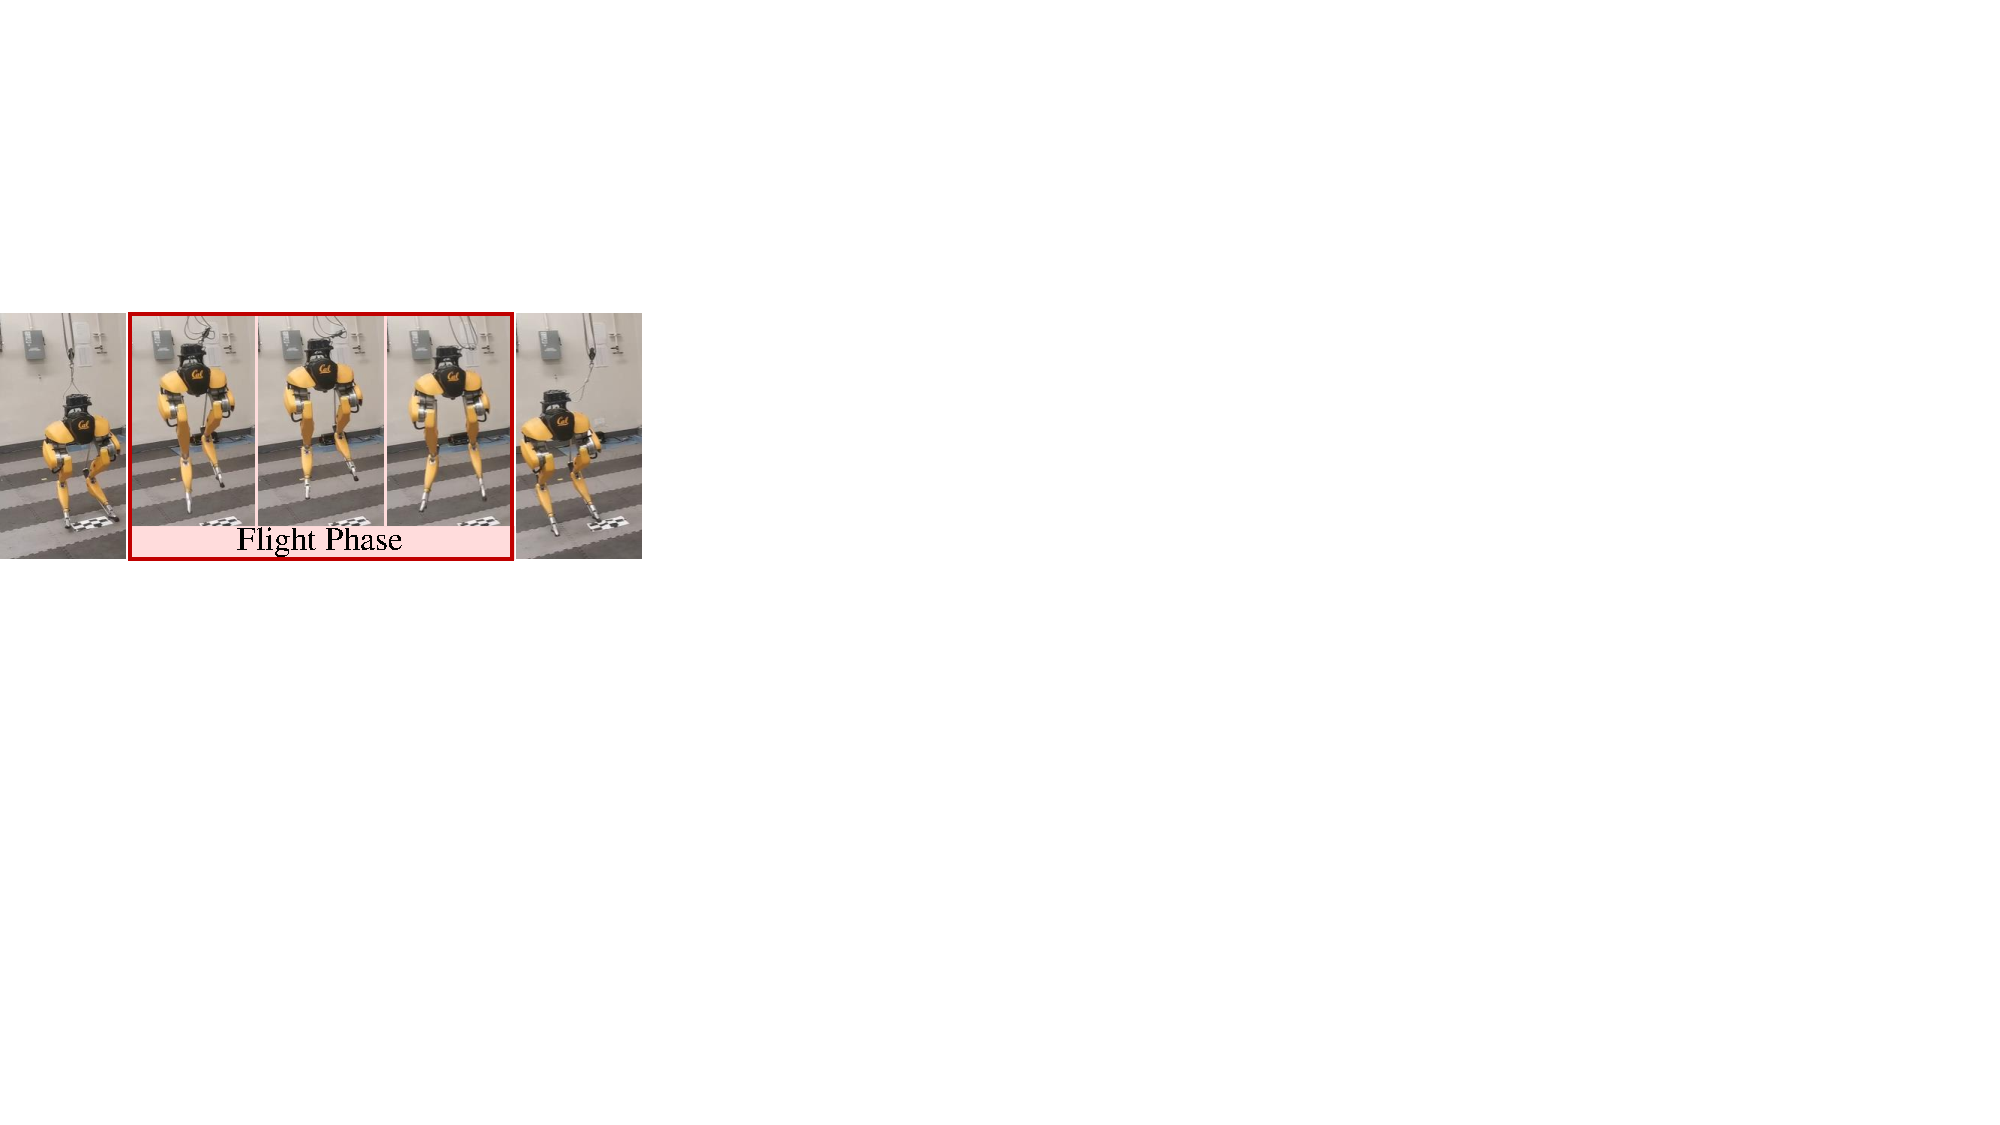
\includegraphics[width=\linewidth]{figures/jump_snapshot_lateral.pdf}
  \caption{$(q^d_x, q^d_y, q^d_\phi)$ = (0m, -0.3m, 0$^\circ$)}
  \label{subfig:jump_flat_lat03}
\end{subfigure}
\begin{subfigure}{0.67\linewidth}
  \centering
  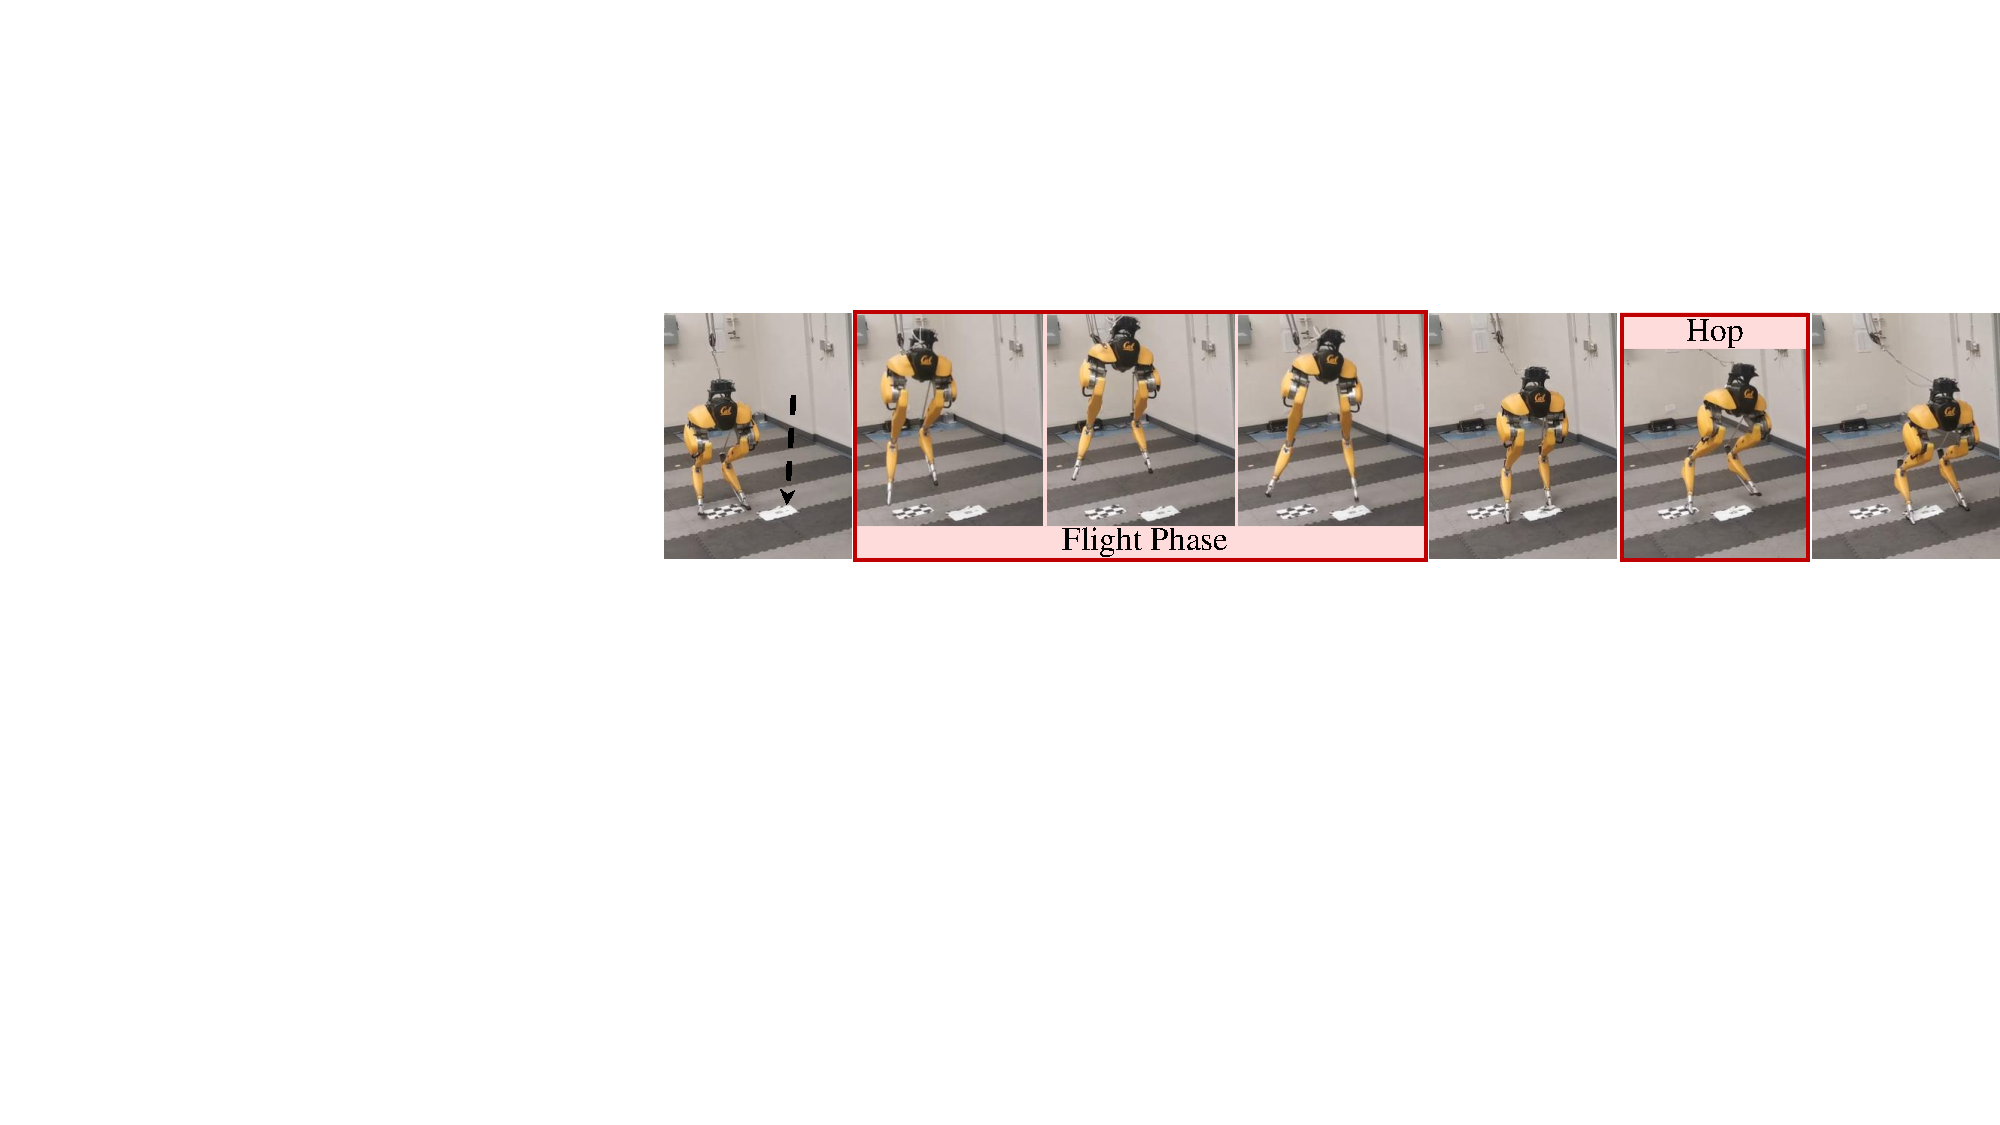
\includegraphics[width=\linewidth]{figures/jump_snapshot_saggital_lateral.pdf}
  \caption{$(q^d_x, q^d_y, q^d_\phi)$ = (0.3m, 0.3m, 0$^\circ$)}
  \label{subfig:jump_flat_lat03sag03}
\end{subfigure}
\begin{subfigure}{\linewidth}
  \centering
  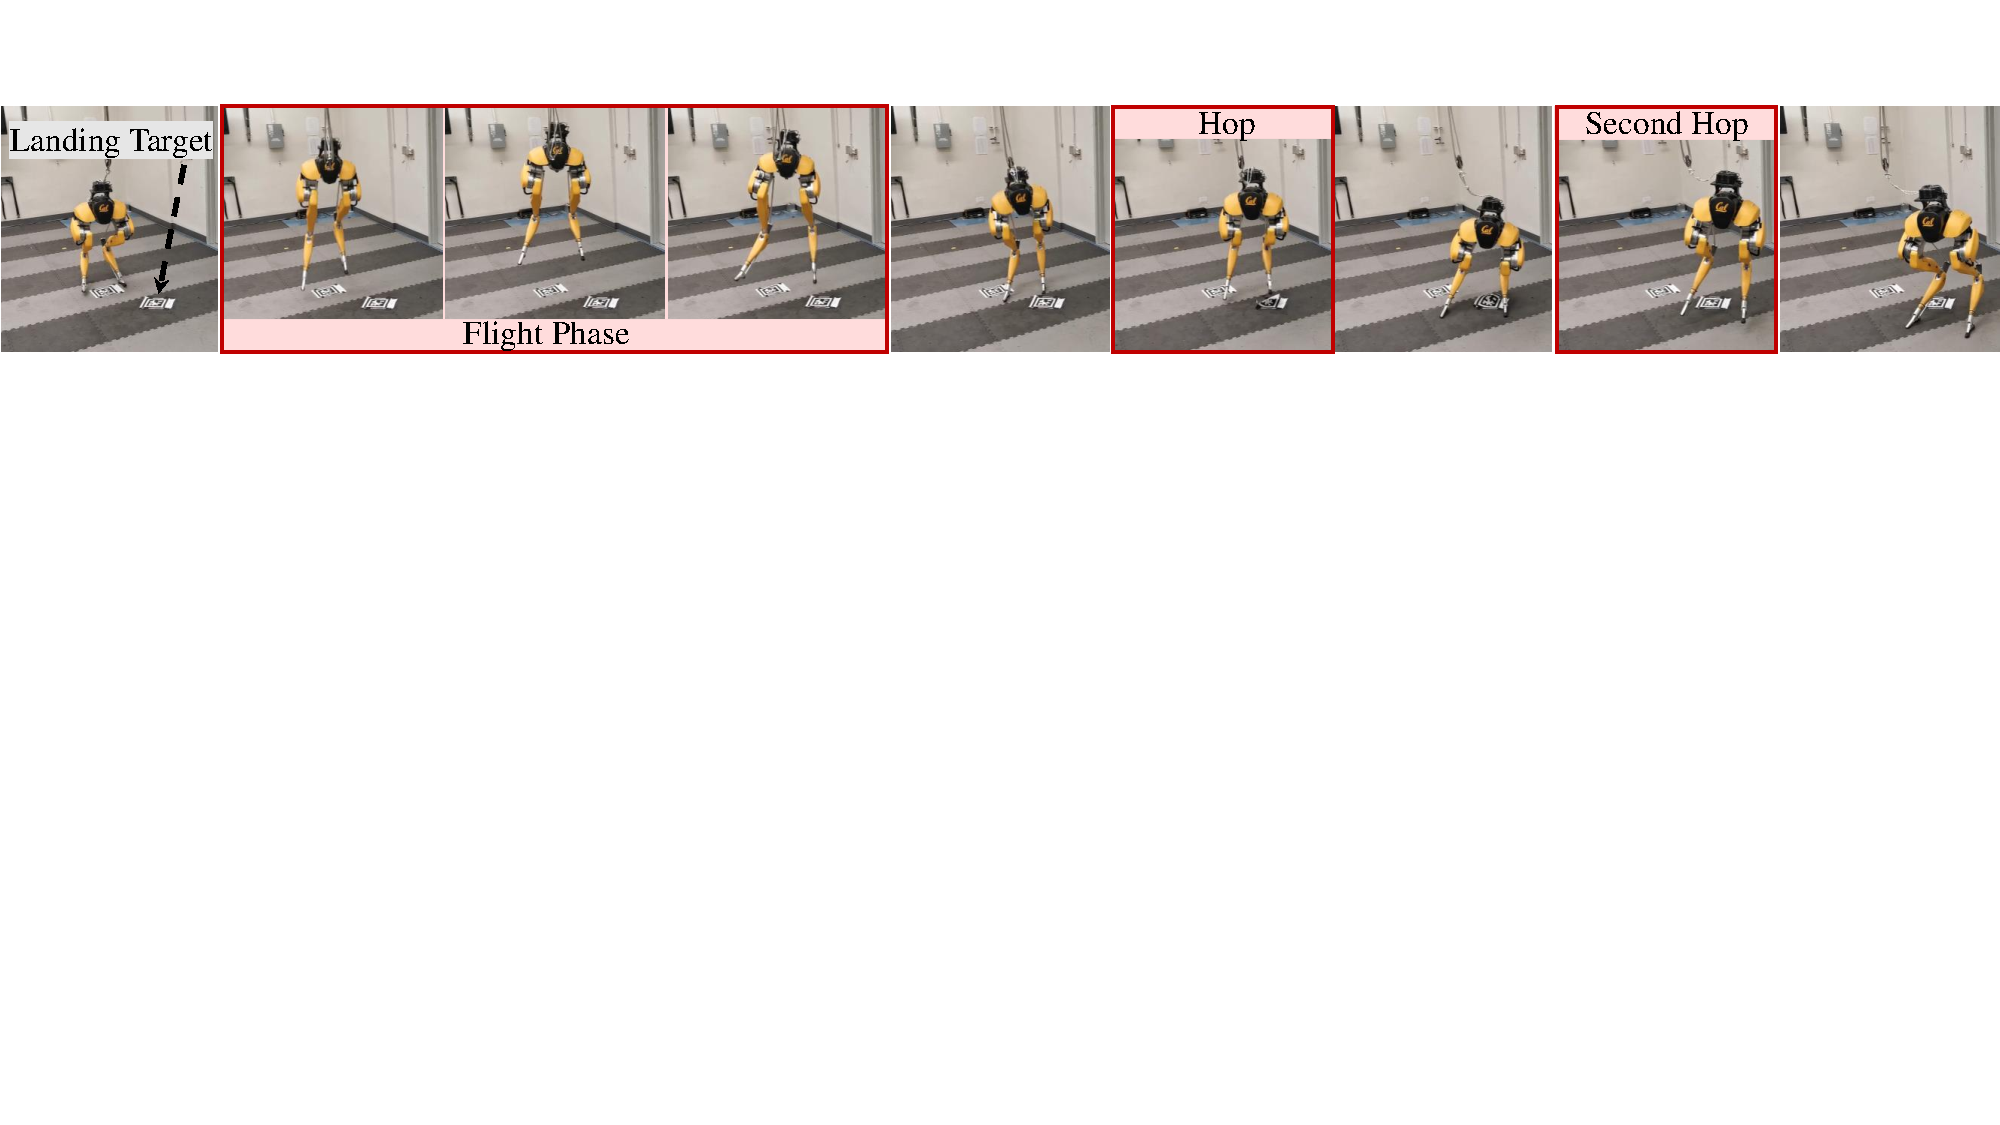
\includegraphics[width=\linewidth]{figures/jump_snapshot_mutliaxes.pdf}
  \caption{$(q^d_x, q^d_y, q^d_\phi)$ = (0.5m, 0.2m, -45$^\circ$)}
  \label{subfig:jump_flat_multiaxes}
\end{subfigure}
\begin{subfigure}{0.345\linewidth}
  \centering
  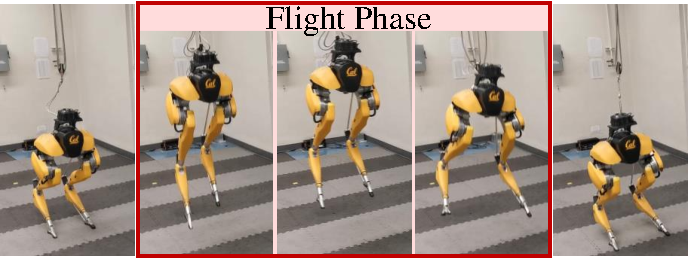
\includegraphics[width=\linewidth]{figures/jump_snapshot_table_inplace.pdf}
  \caption{$(q^d_x, q^d_z)$ = (0m, 0m)}
  \label{subfig:jump_table_inplace}
\end{subfigure}
\begin{subfigure}{0.647\linewidth}
  \centering
  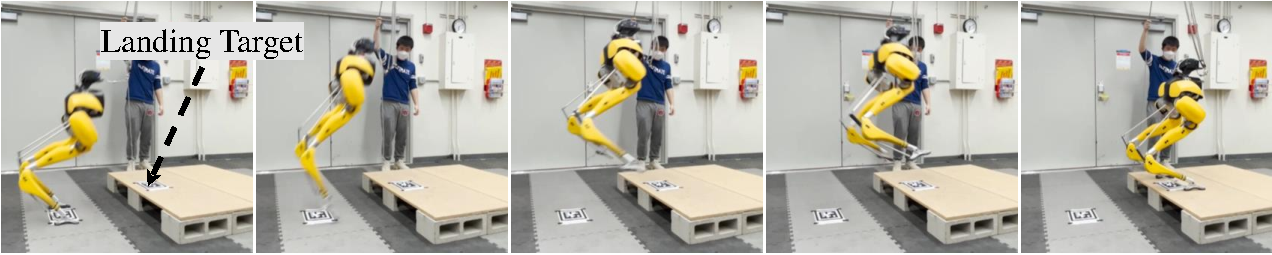
\includegraphics[width=\linewidth]{figures/jump_snapshot_table_014.pdf}
  \caption{$(q^d_x, q^d_z)$ = (0.88m, 0.17m)}
  \label{subfig:jump_table_088017}
\end{subfigure}
\begin{subfigure}{0.495\linewidth}
  \centering
  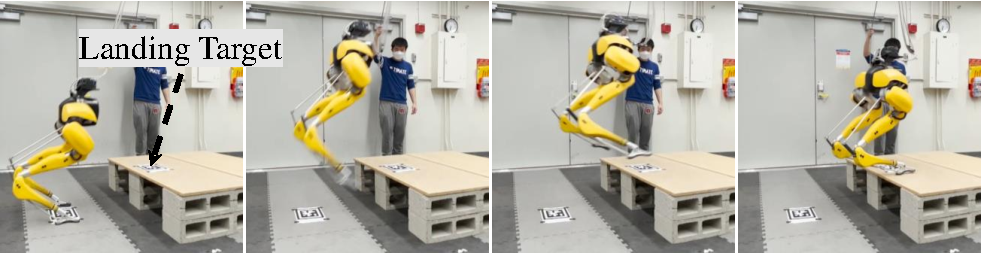
\includegraphics[width=\linewidth]{figures/jump_snapshot_table_032088.pdf}
  \caption{$(q^d_x, q^d_z)$ = (0.88m, 0.32m)}
  \label{subfig:jump_table_088032}
\end{subfigure}
\begin{subfigure}{0.495\linewidth}
  \centering
  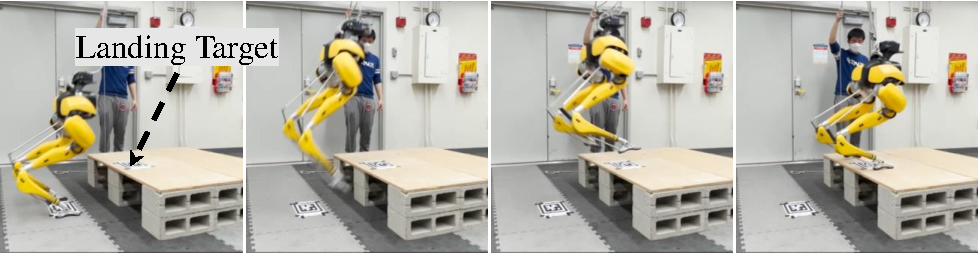
\includegraphics[width=\linewidth]{figures/jump_snapshot_table_032064.pdf}
  \caption{$(q^d_x, q^d_z)$ = (0.64m, 0.32m)}
  \label{subfig:jump_table_064032}
\end{subfigure}
    \caption{Snapshots of more diverse bipedal jumps using the proposed versatile jumping policies. The paper tag on the ground indicates the landing target. Using the same flat-ground policy used in Fig.~\ref{subfig:snapshot_flatx3}, the robot is also able to perform a lateral jump (0.3m to its right in Fig.~\ref{subfig:jump_flat_lat03}), diagonal jump (0.3m ahead and 0.3m to its left in Fig.~\ref{subfig:jump_flat_lat03sag03}), and a complex jumping maneuver that blends forward (0.5m), lateral (0.2m) and turning ($-\text{45}^\circ$) at the same time (Fig.~\ref{subfig:jump_flat_multiaxes}). Using the same discrete-terrain policy used in Fig.~\ref{subfig:snapshot_tablex3}, the robot can also jump in place (Fig.~\ref{subfig:jump_table_inplace}), jump to targets that are placed (Fig.~\ref{subfig:jump_table_088017}) 0.88-meter ahead and 0.17-meter above, (Fig.~\ref{subfig:jump_table_088032}) 0.88-meter ahead and 0.32-meter above, and (Fig.~\ref{subfig:jump_table_064032}) 0.64-meter ahead and 0.32-meter above, respectively.}    
\label{fig:various_jump}
\end{figure*}

We first assess the performance of the \emph{flat-ground} policy, as documented in Fig.~\ref{subfig:snapshot_flatx3}. 
Using this single jumping policy, the robot executes various given target jumps, such as jumping in place while turning $60^\circ$ (Fig.~\ref{subfig:snapshot_flatx3}i), jumping backward to land 0.3-meter behind (Fig.~\ref{subfig:snapshot_flatx3}ii), and jumping to a target placed 1 meter ahead (Fig.~\ref{subfig:snapshot_flatx3}iii), by just changing the command to the policy.
The robot is able to accomplish the task by landing precisely on the target which is marked as a paper tag on the ground. 
Upon closer observation, the robot can adjust its take-off pose in order to follow different commands. 
For instance, it leans backward when required to land on the rear target, and leans forward when executing a forward jump.
The robot is also capable of executing a more diverse set of jumps that combine movements along different axes. 
For instance, Fig.~\ref{subfig:jump_flat_multiaxes} records a representatitve jump where the robot performs a multi-axes jump where it's required to jump forward, laterally, and make a turn at the same time. 
We report more diverse types of jumps (12 different jumps in total) in Appendix~\ref{appendix:other_jumps} and Vid. 5 in Table~\ref{tab:video_list}, and all of these jumps are realized by this single flat-ground jumping policy.


\begin{figure*}[t]
\centering
\begin{subfigure}{0.72\linewidth}
  \centering
  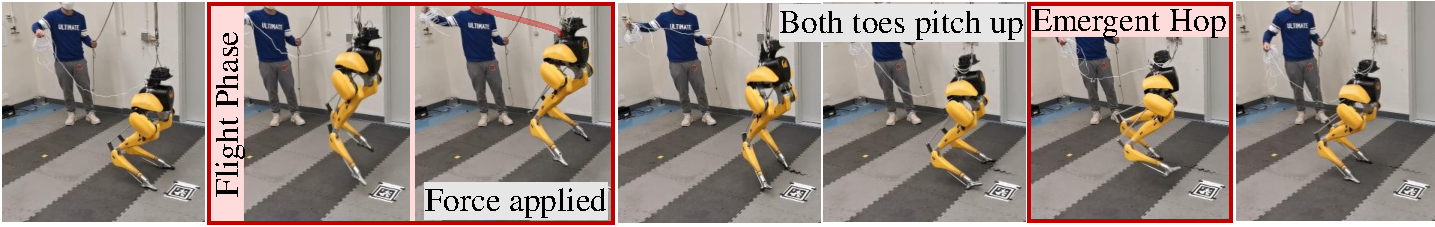
\includegraphics[width=\linewidth]{figures/jump_inplace_perturb.pdf}
  \caption{$(q^d_x, q^d_y, q^d_\psi)$ = (0m, 0m, 0$^\circ$), with perturbation force applied during flight.}
  \label{subfig:jump_inplace_perturb}
\end{subfigure}
\begin{subfigure}{0.2735\linewidth}
  \centering
  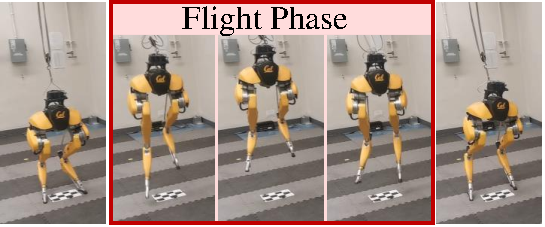
\includegraphics[width=\linewidth]{figures/jump_inplace.pdf}
  \caption{$(q^d_x, q^d_y, q^d_\psi)$ = (0m, 0m, 0$^\circ$)}
  \label{subfig:jump_inplace}
\end{subfigure}
\caption{Snapshots of the robustness test during jumping using the versatile flat-ground policy. In Fig.~\ref{subfig:jump_inplace_perturb}, an unexpected backward perturbation is applied while at its apex height during an in-place jump. This contrasts with Fig.~\ref{subfig:jump_inplace}, where the robot performs the same task without perturbation, serving as a baseline. Despite leaning backward upon landing due to the perturbation, the robot spontaneously executes a backward hop, a maneuver it learned during other tasks like backward jumping, and succeeds to maintain balance after landing. Such a robustness is achieved through \textit{task randomization} alone, as the jumping policy was not trained with simulated perturbation.}    
\label{fig:jump_perturb}
\end{figure*}

\subsubsection{Jump to Elevated Platforms}
We then evaluate the \emph{discrete-terrain} policy to control the robot's jumping ability over various distances and elevations. 
As showcased in Fig.~\ref{subfig:snapshot_tablex3}, the robot exhibits the capability to jump precisely to targets placed at different positions, like 1 meter ahead (Fig.~\ref{subfig:snapshot_tablex3}iii) or 1.4 meters ahead (Fig.~\ref{subfig:snapshot_tablex3}ii), and at varying elevations, including 0.44 meters elevated (Fig.~\ref{subfig:snapshot_tablex3}i, considering the robot height is only 1.1 meter). 
Using the single discrete-terrain policy, the robot is able to adjust its take-off maneuvers for different jumping targets and efficiently manages its angular momentum after the large impact upon landing to maintain stability. 
In addition to standing long jumps (1.4 meters forward) and standing high jumps (0.44 meters elevated), we conducted a range of varied jumping tasks within this range, including jumping in place (with foot clearance around 0.4 meters at its apex height) and jumping over different sagittal distances onto various elevated platforms. 
These tasks were all conducted using the same policy, as shown in Fig.~\ref{fig:various_jump}.
Notably, the standing long jump over 1.4 meters and standing high jump to a 0.44-meter elevated platform (while using the same controller) are the novel locomotion capacities in the human-sized bipedal robot regime.


\subsubsection{Robust Jumping Maneuvers}
We illustrate the robustness of the jumping policy obtained from the proposed method with an example shown in Fig.~\ref{fig:jump_perturb}. Employing the \emph{flat-ground} policy, we commanded the robot to perform an in-place jump. 
At the apex of the jump, we applied a backward impulse perturbation, as depicted in Fig.~\ref{subfig:jump_inplace_perturb}.
This significant perturbation caused the robot to deviate from its nominal in-place jumping trajectory (as seen in Fig.~\ref{subfig:jump_inplace}), resulting in a significant change in its pose upon landing. Consequently, the robot landed with a backward lean and its toes pitched up trying to stabilize the robot. 
This pose presented a significant challenge, given that the robot became underactuated and was nearly losing balance.
However, since the jumping policy has been trained to execute backward jumps, as previously showcased in Fig.~\ref{subfig:snapshot_flatx3}ii, the robot rapidly adjusted its intended landing trajectory and executed a backward hop. By this adjustment, the robot is able to better correct its pose in the air to achieve a more favorable configuration upon its next landing. 

Note that the jumping policies were never trained explicitly to handle perturbations. 
Therefore, this experiment highlights the advantage of a versatile jumping policy. 
The robot demonstrates the ability to generalize its learned diverse tasks to devise a better maneuver and contact plan rather than strictly adhering to the given task during real-world deployment. 
This serves as a detailed report of successful recovery from a perturbation while a bipedal robot is executing a jump in the real world, illustrating the importance of the \textit{task randomization}.



\begin{remark}
Using versatile policies for walking, running, and jumping, the robot exhibits the capability to develop its own contact strategy online, deviating from the contact plans (implicitly) provided by reference motions. This ability enhances stability and robustness. For instance, in jumping experiments, the robot often breaks contact after landing and executes small hops to achieve a better landing configuration, as seen in Fig.~\ref{fig:jump_perturb}.
This capacity is also evident in other skills, such as standing (Fig.~\ref{subfig:bm_multi_walking}), walking (with significant double-support phases contrary to the single-support in reference motions, as in Fig.~\ref{subfig:walking_slope}), and running (where the robot does not strictly follow the contact sequence of the periodic running reference motion, as seen in Fig.~\ref{fig:100run}).
This emergent capability aligns with what contact-implicit optimization, like in \cite{posa2014direct,drnach2021robust,landry2022bilevel}, aims to achieve. While these piror methods have only achieved such optimization offline for bipedal robots, our work realizes this online on a real bipedal robot.
\end{remark}


\begin{remark}
We note that during the jumping experiments, the robot occasionally oscillates while standing after a large jump. 
This is due to the challenges of learning a single RL policy to learn both dynamic aperiodic jumping skill and stationary standing skill. 
The features learned during a jump may favor high-acceleration motion and cannot easily alter the policy's behavior for perfectly stationary standing. 
This also provides an insight into the challenges of obtaining a single unified policy to learn all different locomotion skills (to combine dynamic and stationary skills). 
But we want to note that, the jumping policy is still able to damp out such an oscillation during standing, though with a longer noticeable time, as demonstrated in the supplementary video (Vid. 5). 
\end{remark}


\subsubsection{Summary of Results}
We demonstrated 19 distinct bipedal jumps in the real world, encompassing a range of landing locations, turns, and elevations. 
These jumps were conducted using just two versatile policies: the \emph{flat-ground} policy and the \emph{discrete-terrain} policy.
Through these extensive real-world experiments, we illustrated two key aspects of the proposed method, using the jumping skill as an exemplary case. 
First, we showcase the \emph{adaptivity} of the proposed policy. 
The robot exhibits the capability to land precisely on a designated target after a flight phase, all without requiring global position feedback. 
To achieve this, the robot must generate a precise amount of momentum at take-off. 
By accomplishing these diverse jumping tasks, the RL-based control policy showcases its adaptivity to the robot's hardware dynamics, mainly by leveraging the long-term I/O history, to control the robot and achieve accurate take-off translational velocities to land at the target.
Second, we highlight the \emph{robustness} of the policy. 
Despite being trained without perturbation, the robot demonstrates an ability to respond to unexpected perturbations during jumping by employing learned tasks for agile recovery.